\documentclass[a4paper]{article}
\usepackage[margin=3.5cm]{geometry}
\usepackage{amsmath,amsfonts,amssymb,amsthm}
\usepackage{thmtools, thm-restate}
\usepackage[svgnames]{xcolor}
\usepackage{graphicx}
\usepackage{dsfont}
\usepackage{hyperref}
\usepackage{datetime}
\usepackage{outlines}
\usepackage{float}
\usepackage{booktabs}
\usepackage{enumitem}
\usepackage{outlines}


\definecolor{fgcolor}{rgb}{0.345, 0.345, 0.345}
\newcommand{\hlnum}[1]{\textcolor[rgb]{0.686,0.059,0.569}{#1}}%
\newcommand{\hlstr}[1]{\textcolor[rgb]{0.192,0.494,0.8}{#1}}%
\newcommand{\hlcom}[1]{\textcolor[rgb]{0.678,0.584,0.686}{\textit{#1}}}%
\newcommand{\hlopt}[1]{\textcolor[rgb]{0,0,0}{#1}}%
\newcommand{\hlstd}[1]{\textcolor[rgb]{0.345,0.345,0.345}{#1}}%
\newcommand{\hlkwa}[1]{\textcolor[rgb]{0.161,0.373,0.58}{\textbf{#1}}}%
\newcommand{\hlkwb}[1]{\textcolor[rgb]{0.69,0.353,0.396}{#1}}%
\newcommand{\hlkwc}[1]{\textcolor[rgb]{0.333,0.667,0.333}{#1}}%
\newcommand{\hlkwd}[1]{\textcolor[rgb]{0.737,0.353,0.396}{\textbf{#1}}}%
\let\hlipl\hlkwb

\usepackage{framed}
\makeatletter
\newenvironment{kframe}{%
 \def\at@end@of@kframe{}%
 \ifinner\ifhmode%
  \def\at@end@of@kframe{\end{minipage}}%
  \begin{minipage}{\columnwidth}%
 \fi\fi%
 \def\FrameCommand##1{\hskip\@totalleftmargin \hskip-\fboxsep
 \colorbox{shadecolor}{##1}\hskip-\fboxsep
     % There is no \\@totalrightmargin, so:
     \hskip-\linewidth \hskip-\@totalleftmargin \hskip\columnwidth}%
 \MakeFramed {\advance\hsize-\width
   \@totalleftmargin\z@ \linewidth\hsize
   \@setminipage}}%
 {\par\unskip\endMakeFramed%
 \at@end@of@kframe}
\makeatother

\definecolor{shadecolor}{rgb}{.97, .97, .97}
\definecolor{messagecolor}{rgb}{0, 0, 0}
\definecolor{warningcolor}{rgb}{1, 0, 1}
\definecolor{errorcolor}{rgb}{1, 0, 0}
\newenvironment{knitrout}{}{} % an empty environment to be redefined in TeX


% code highlighting
\usepackage{minted}
\usepackage{xpatch}
\newminted[cminted]{python}{fontsize=\small}
\xpretocmd{\cminted}{\RecustomVerbatimEnvironment{Verbatim}{BVerbatim}{}}{}{}

% link coloring
%\hypersetup{
%    colorlinks,
%    linkcolor={red!80!black},
%    citecolor={green!60!black},
%    urlcolor={blue!80!black}
%}

% concatenation symbol (c.f. ++ in Haskell)
\newcommand\mdoubleplus{\mathbin{+\mkern-10mu+}}

% end of proof symbol
\newcommand{\newmarkedtheorem}[1]{%
  \newenvironment{#1}
    {\pushQED{\qed}\csname inner@#1\endcsname}
    {\popQED\csname endinner@#1\endcsname}%
  \newtheorem{inner@#1}%
}

\theoremstyle{definition}
%\newtheorem{eg}{Example}[section]
\newmarkedtheorem{eg}{Example}[section]
\newtheorem{observation}{Observation}[section]
\newtheorem{define}{Definition}[section]
\theoremstyle{plain}
\newtheorem{proposition}{Proposition}
\newtheorem{lemma}{Lemma}
\newtheorem{corollary}{Corollary}
\newtheorem{theorem}{Theorem}[section]
\newtheorem{assump}{Assumption}[section]
\newtheorem{remark}{Remark}[section]

\newdateformat{monthyeardate}{\monthname[\THEMONTH] \THEYEAR}

\author{Jeroen van Riel}
\date{\monthyeardate\today}
\title{Trajectory Optimization of Autonomous Vehicles in a Single Intersection}

\begin{document}

\maketitle

\tableofcontents


\section{Background}


\subsection{Job-shop scheduling}

\paragraph{Constructive heuristics}
A common approach for developing such heuristics found in the scheduling
literature is to try and construct a good schedule in a step-by-step fashion, to
which may be called \textit{constructive heuristics}. For the crossing time
scheduling problem, we may consider methods that incrementally construct a
vehicle ordering.

\subsection{Reinforcement learning}

Generally speaking, RL methods that use the current learned policy for data
collection are referred to as \textit{on-policy} methods, methods that use a
fixed separate policy for data collection are referred to as
\textit{off-policy}.


\section{Problem definition and decomposition}

\begin{figure}
  \centering
  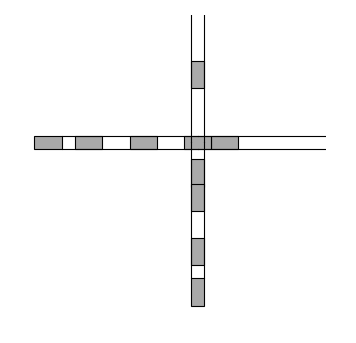
\includegraphics[width=0.4\textwidth]{figures/single/single_intersection_example.png}
  \caption{Illustration of a single intersection with vehicles drawn as grey
    rectangles. Vehicles approach the intersection from the east and from the
    south and cross it without turning. Note that the first two waiting vehicles
    on the south lane kept some distance before the intersection, such that they
    are able to reach full speed whenever they
    cross.}\label{fig:intersection_illustration}
\end{figure}

% general model: multi-agent optimal control problem
% derivation of the following ``offline trajectory optimization problem for a single intersection'' should happen elsewhere
% reiterate assumptions:
% (0. single intersection)
% 1. all future arrivals known
% 2. fixed routes (no dynamic rerouting)
% 3. vehicle dynamics: double integrator
% 4. central controller
We start by defining the \textit{vehicle trajectory optimization problem} for a
single intersection.
%
Consider the single intersection illustrated in
Figure~\ref{fig:intersection_illustration}, which has two incoming lanes,
identified by indices $\mathcal{R} = \{ 1, 2 \}$. The corresponding two routes
are crossing the intersection from south to north and crossing from west to
east.
%
Each route is followed by a fixed set of vehicles, so we consider a closed
system, in the sense that no more vehicles arrive in the future.
%
We identify vehicles by their route and by their relative order on this
route, by defining the vehicle index set
\begin{align}
  \mathcal{N} = \{ (r, k) : k \in \{1, \dots, n_{r}\}, r \in \mathcal{R}\} ,
\end{align}
where $n_{r}$ denotes the number of vehicles following route $r$. Smaller
values of $k$ correspond to reaching the intersection earlier. Given vehicle
index $i = (r, k) \in \mathcal{N}$, we also use the notation $r(i) = r$ and
$k(i) = k$.
%
We assume that each vehicle is represented as a rectangle of length $L_{i}$ and
width $W_{i}$ and we define its longitudinal position $x_{i}(t)$ along its route
to be the distance between its front bumper and the start of the lane. The
position of a vehicle over time is governed by the well-known \textit{double integrator}
model
\begin{gather}
  \label{eq:vehicle_dynamics}
\begin{aligned}
  \dot{x}_{i}(t) = v_{i}(t) , \\
  \dot{v}_{i}(t) = u_{i}(t)  , \\
  0 \leq v_{\max} \leq v_{\max} , \\
  |u_{i}(t) | \leq a_{\max} ,
\end{aligned}
\end{gather}
where $v_{i}(t)$ is the vehicle's velocity and $u_{i}(t)$ its acceleration. Let
$D_{i}(s_{i,0})$ denote the set of all trajectories $x_{i}(t)$ satisfying these
dynamics, given some initial state $s_{i,0} = (x_{i}(0), v_{i}(0))$.
%
In order to maintain a safe distance between consecutive vehicle on the same
lane, vehicle trajectories need to satisfy the \textit{safe headway constraints}
\begin{align}
  \label{eq:follow_constraints}
  x_{i}(t) - x_{j}(t) \geq L_{i} ,
\end{align}
for all $t$ and all pairs of indices $i, j \in \mathcal{N}$ such that
$r(i) = r(j), k(i) + 1 = k(j)$. Let $\mathcal{C}$ denote the set of such ordered
pairs of indices. Note that these constraints restrict vehicle from overtaking
each other, so the initial relative order is always maintained.
%
For each $i \in \mathcal{N}$, let $\mathcal{E}_{i} = (B_{i}, E_{i})$ denote the
open interval such that vehicle $i$ occupies the intersection's conflict area if
and only if $x_{i}(t) \in \mathcal{E}_{i}$. Using this notation\footnote{Note
  that it would make sense to let $B_{i}$ be equal for all vehicles $i$ that
  follow the same route, which we do not emphasize with the notation to keep it
  simple.}, collision avoidance at the intersection is achieved by requiring
\begin{align}
  \label{eq:conflict_constraints}
  (x_{i}(t), x_{j}(t)) \notin \mathcal{E}_{i} \times \mathcal{E}_{j} ,
\end{align}
for all $t$ and for all pairs of indices $i, j \in \mathcal{N}$ with
$r(i) \neq r(j)$, to which we will refer as the set of \textit{conflicts}, denoted
by $\mathcal{D}$.

Suppose we have some performance criterion $J(x_{i})$ that takes into account
travel time and energy efficiency of the trajectory of vehicle $i$. Suppose
there is some central decision making entity that controls the acceleration of
all vehicles in the system at once, then the trajectory optimization problem for
a single intersection can be compactly written as
\begin{subequations}
\label{eq:offline_single_intersection}
\begin{align}
  \min_{x} \quad & \sum_{i \in \mathcal{N}} J(x_{i}) \\
  \text{s.t.} \quad  & x_{i} \in D_{i}(s_{i,0}) , &\text{for all } i \in \mathcal{N} , \\
                & x_{i}(t) - x_{j}(t) \geq L_{i}, &\text{for all } (i,j) \in \mathcal{C} , \\
                & (x_{i}(t), x_{j}(t))  \notin \mathcal{E}_{i} \times \mathcal{E}_{j} , &\text{for all } \{i,j\} \in \mathcal{D} \label{eq:collision_constraints} ,
\end{align}
\end{subequations}
where all constraints apply at all times $t$.


\subsection{Direct transcription}

Although computationally demanding,
problem~\eqref{eq:offline_single_intersection} can be numerically solved by
direct transcription to a non-convex mixed-integer linear program by
discretization on a uniform time grid. Let $K$ denote the number of discrete
time steps and let $\Delta t$ denote the time step size.
%
Using the forward Euler integration scheme, we have
\begin{align*}
  x_{i}(t + \Delta t) = x_{i}(t) + v_{i}(t) \Delta t , \\
  v_{i}(t + \Delta t) = v_{i}(t) + u_{i}(t) \Delta t ,
\end{align*}
for each $t \in \{0, \Delta t, \dots, K \Delta t\}$. Following the approach in~\cite{hultApproximateSolutionOptimal2015}, the
collision-avoidance constraints between lanes can be formulated using the
well-known big-M technique with binary decision variables, by defining the
constraints
\begin{align*}
  x_{i}(t) \leq B_{i} + \delta_{i}(t) M , \\
  E_{i} - \gamma_{i}(t) M \leq x_{i}(t) , \\
  \delta_{i}(t) + \delta_{j}(t) + \gamma_{i}(t) + \gamma_{j}(t) \leq 3 ,
\end{align*}
where $\delta_{i}(t), \gamma_{i}(t) \in \{ 0, 1 \}$ for all $i \in \mathcal{N}$ and $M$ is some
sufficiently large number.
%
Finally, the safe headway constraints can simply be added as
\begin{align*}
  x_{i}(t) - x_{j}(t) \geq L_{i} ,
\end{align*}
for each $t \in \{0, \Delta t, \dots, K \Delta t\}$ and each pair of consecutive
vehicles $(i, j) \in \mathcal{C}$ on the same lane.
%
To illustrate the method, consider the objective functional
\begin{align*}
  J(x_{i}) = \int_{t=0}^{t_{f}} \left( {(v_{d} - v_{i}(t))}^{2} + {u_{i}(t)}^{2} \right) dt ,
\end{align*}
where $v_{d}$ is some reference velocity and $t_{f}$ denotes the final time.
This objective can be roughly interpreted as trying to maintain a velocity close
to $v_{d}$, while simultaneously minimizing the energy consumption required for
acceleration and deceleration. For a problem with five identical vehicles with
initial conditions as given in Table~\ref{tab:hult_parameters}, the optimal
trajectories are shown in Figure~\ref{fig:direct_transcription_example}.

\definecolor{armygreen}{rgb}{0.29, 0.33, 0.13}
\begin{table}[H]
  \centering
\begin{tabular}{ c | c c c | c c }
  $i$  & {\color{armygreen}(1,1)} & {\color{armygreen}(1,2)} & {\color{armygreen}(1,3)} & {\color{red}(2,1)} & {\color{red}(2,2)} \\
  \hline
  $x_{i}(0)$ & 15 & 10 &  0 & 10 &  0 \\
  $v_{i}(0)$ & 10 & 10 &  6 & 12 & 10 \\
\end{tabular}
\caption{Example of initial states $s_{i,0} = (x_{i}(0), v_{i}(0))$ for
  problem~\eqref{eq:offline_single_intersection} with five identical vehicles.}
\label{tab:hult_parameters}
\end{table}

\begin{figure}[H]
  \centering
  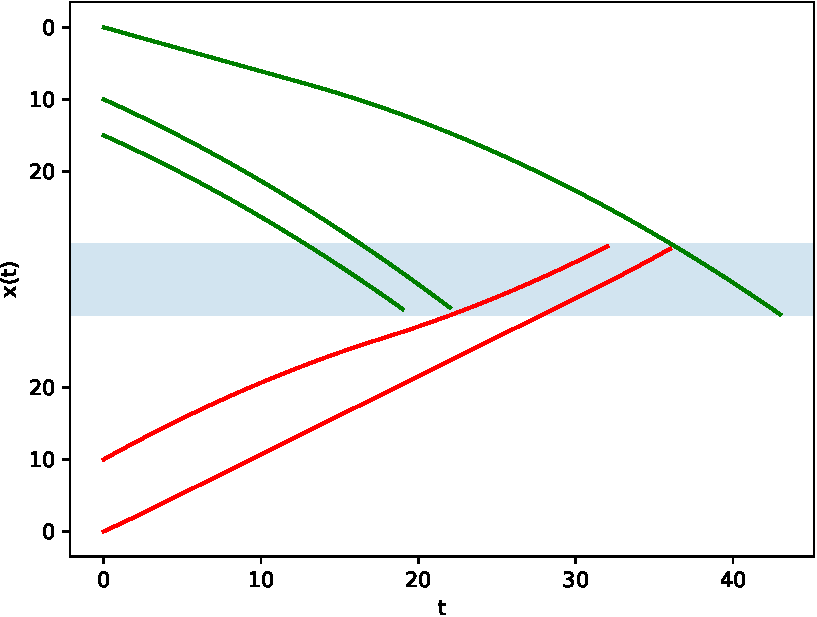
\includegraphics[width=0.8\textwidth]{figures/single/trajectories_general.pdf}
  \caption{Example of optimal trajectories obtained using the direct
    transcription method with
    $L_{i} \equiv L = 5, \, \mathcal{E}_{i} \equiv \mathcal{E} = [50, 70], \, v_{d} = 20, \; T=120, \, \Delta t = 0.1$
    and initial conditions as given in Table~\ref{tab:hult_parameters}. The
    y-axis is split such that each part corresponds to one of the two lanes and
    the trajectories are inverted accordingly and drawn with separate colors.
    The intersection area $\mathcal{E}$ is drawn as a shaded region. Whenever a
    vehicle has left the intersection, we stop drawing its trajectory for
    clarity.}
  \label{fig:direct_transcription_example}
\end{figure}


\subsection{General decomposition}

For the case where only a single vehicle is approaching the intersection for
each route, so $n_{r} = 1$ for each route $r \in \mathcal{R}$, it has been shown
that problem~\eqref{eq:offline_single_intersection} can be decomposed into two coupled optimization problems, see
Theorem 1 in~\cite{hultApproximateSolutionOptimal2015}. Roughly speaking, the \textit{upper-level problem} optimizes the time
slots during which vehicles occupy the intersection, while the \textit{lower-level problem}
produces optimal safe trajectories that respect these time slots.
%
When allowing multiple vehicles per lane, we show without proof that a similar
decomposition is possible.
%
Given $x_{i}(t)$, the \textit{crossing time} of vehicle $i$, when the vehicle
first enters the intersection, and the corresponding \textit{exit time} are respectively
\begin{align*}
  \inf \{ t: x_{i}(t) \in \mathcal{E}_{i} \}  \;\; \text{ and } \; \sup \{ t: x_{i}(t) \in \mathcal{E}_{i} \} .
\end{align*}
%
The upper-level problem is to find a set of feasible occupancy timeslots, for
which the lower-level problem generates trajectories. The trajectories can be
generated separately for each route, which leads to some degree of decomposition
of the problem.
%
We will use decision variable $y_{i}$ for the crossing time and write
$y_{i} + \sigma_{i}$ for the exit time, so $\sigma_{i}$ is the amount of time vehicle
$i$ occupies the intersection. Let
$\mathcal{N}_{r} = \{ i \in \mathcal{N} : r(i) = r\}$ be all vehicles on route
$r$ and write vector $y_{r} = [ y_{i} : i \in \mathcal{N}_{r} ]$ and similarly
define ${\sigma}_{r}$, ${x}_{r}$ and ${s}_{r,0}$.
%
Using this notation, the problem can be decomposed into the upper-level
\textit{crossing time scheduling} problem
%
\begin{align*}
  \min_{{y}, {\sigma}} \quad & \sum_{r \in \mathcal{R}} F({y}_{r}, {\sigma}_{r}) \\
  \text{ s.t. } \quad & y_i + \sigma_i \leq y_j \text{ or } y_j + \sigma_j \leq y_i, & \text{ for all } \{i, j\} \in \mathcal{D} , \\
  & ({y}_{r}, {\sigma}_{r}) \in \mathcal{S}_{r} , & \text{ for all } r \in \mathcal{R} ,
\end{align*}
where $F({y}_{r}, {\sigma}_{r})$ and $\mathcal{S}_{r}$ are the value function and set of
feasible parameters, respectively, of the lower-level \textit{route trajectory optimization}
problem
\begin{align*}
  F({y}_{r}, {\sigma}_{r}) = \min_{{x}} \quad & \sum_{i \in \mathcal{N}_{r}} J(x_{i}) \\
  \text{ s.t. } \quad & x_{i} \in D_{i}(s_{i,0}) , & \text{ for all } i \in \mathcal{N}_{r} , \\
  & x_{i}(y_i) = B_{i} , & \text{ for all } i \in \mathcal{N}_{r} , \\
  & x_{i}(y_i + \sigma_i) = E_{i} , & \text{ for all } i \in \mathcal{N}_{r} , \\
  & x_{i}(t) - x_{j}(t) \geq L_{i} , & \text{ for all } (i, j) \in \mathcal{C} \cap \mathcal{N}_{r} .
\end{align*}
Note that the set of feasible parameters $\mathcal{S}_{r}$ implicitly depends on
the initial states ${s}_{r,0}$ and the global system parameters.


\subsection{Decomposition for delay objective}

Assume that the trajectory performance criterion is based on the amount of delay experienced by vehicles.
% earliest time of arrival
Observe that $a_{i} := (B_{i} - x_{i}(0)) / v_{\max}$ is the earliest time at
which vehicle $i$ can enter the intersection, so we will define the delay of
vehicle $i$ to be $J(x_{i}) = y_i - a_{i}$. This assumption makes the problem
significantly simpler, because we now have
\begin{align*}
  F(y_{r}, \sigma_{r}) \equiv F(y_{r}) = \sum_{i \in \mathcal{N}_{r}} y_i - a_{i}.
\end{align*}
%
Furthermore, we assume that vehicles have full speed initially and when crossing
the intersection, so $v_{i}(0) = v_{i}(y_i) = v_{\max}$, and we assume that all
vehicles are identical, so $L_{i} = L$ and $W_{i} = W$ for all
$i \in \mathcal{N}$, such that we have
\begin{align*}
\sigma(i) \equiv \sigma = (L + W) / v_{\max}, \; \text{ for all } i \in \mathcal{N} .
\end{align*}
%
Therefore, we ignore the part related to $\sigma$ in the set of feasible parameters
$\mathcal{S}_{r}$, which can be shown that to have a particularly simple
structure under these assumptions.
% processing time
Let $\rho := L / v_{\max}$ be such that $y_i + \rho$ is the time at which the rear
bumper of a crossing vehicle reaches the start line of the intersection, to
which we will refer as the \textit{processing time}. It can now be shown that
$y_{r} \in \mathcal{S}_{r}$ holds whenever
\begin{align*}
  a_{i} \leq y_i , & \text{ for all } i \in \mathcal{N}_{r} , \\
  y_i + \rho \leq y_j , & \text{ for all } (i,j) \in \mathcal{C} \cap \mathcal{N}_{r} .
\end{align*}
Therefore, under the stated assumptions, the offline trajectory optimization
problem~\eqref{eq:offline_single_intersection} reduces to the following \textit{crossing time scheduling} problem
\begin{subequations}
  \label{eq:crossing_time_scheduling}
\begin{align}
  \min_{y} \quad & \sum_{i \in \mathcal{N}} y_i - a_{i} \\
  \text{ s.t. } \quad & a_{i} \leq y_i , & \text{ for all } i \in \mathcal{N} , \\
                    & y_i + \rho \leq y_{j} , & \text{ for all } (i,j) \in \mathcal{C} \label{eq:conjunctive} , \\
                    & y_i + \sigma \leq y_{j} \text{ or } y_j + \sigma \leq y_i , & \text{ for all } \{i,j\} \in \mathcal{D} \label{eq:disjunctive} .
\end{align}
\end{subequations}
This problem can be solved using off-the-shelf mixed-integer linear program solvers,
after encoding the \textit{disjunctive constraints}~\eqref{eq:disjunctive} using
the big-M technique, which we will demonstrate in
Section~\ref{sec:branch-and-cut}. Given optimal crossing time schedule $y^{*}$, any set of trajectories
$[x_{i}(t) : i \in \mathcal{N}]$ that satisfies
\begin{align*}
  x_{i} \in D_{i}(s_{i,0}) , \quad & \text{ for all } i \in \mathcal{N} , \\
  x_{i}(y^{*}_i) = B_{i} , \quad & \text{ for all } i \in \mathcal{N} , \\
  x_{i}(y^{*}_i + \sigma) = E_{i} , \quad & \text{ for all } i \in \mathcal{N} , \\
  x_{i}(t) - x_{j}(t) \geq L , \quad & \text{ for all } (i,j) \in \mathcal{C} ,
\end{align*}
is a valid solution. These trajectories can be computed with an efficient direct
transcription method. Note that each route may be considered separately, so
trajectories can be computed by solving the time-discretized version of the
optimal control problem
%
\begin{align*}
\texttt{MotionSynthesize}(\tau, B, s_{0}, x') := \\
  {\arg\min}_{x: [0, \tau] \rightarrow \mathbb{R}} & \int_{0}^{\tau} |x(t)| dt \\
  \text{ s.t. } & \ddot{x}(t) = u(t) , &  \text{ for all } t \in [0, \tau] , \\
  & |u(t)| \leq a_{\max} , &  \text{ for all } t \in [0, \tau] , \\
  & 0 \leq \dot{x}(t) \leq v_{\max} , &  \text{ for all } t \in [0, \tau] , \\
  & x'(t) - x(t) \geq L , &  \text{ for all } t \in [0, \tau] , \\
  & (x(0), \dot{x}(0)) = s_{0} , \\
  & (x(\tau), \dot{x}(\tau)) = (B, v_{\max}) ,
\end{align*}
where $\tau$ is the required crossing time, $B$ denotes the distance to
the intersection, $s_{0}$ is the initial state of the vehicle and $x'$ denotes
the trajectory of the vehicle preceding the current vehicle.

\begin{figure}
  \centering
  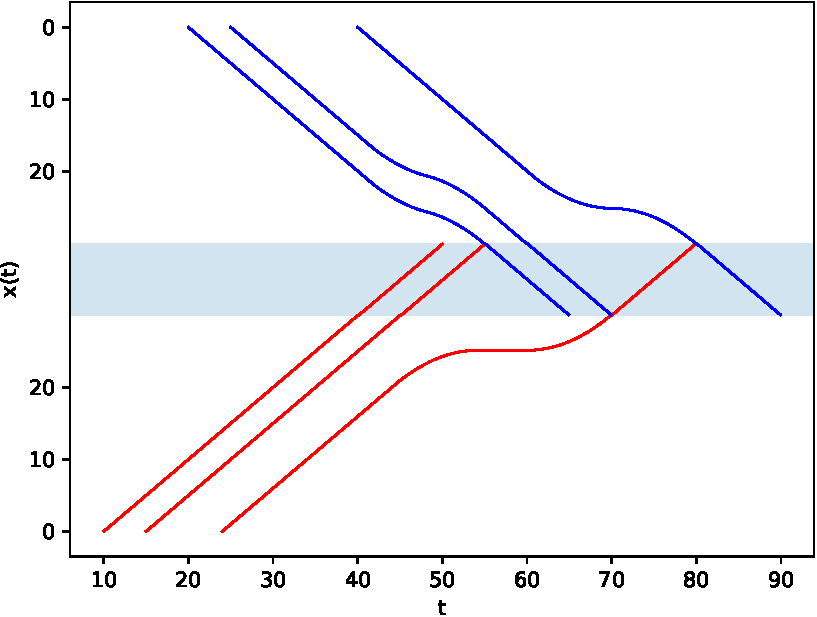
\includegraphics[width=0.8\textwidth]{figures/single/trajectories_delay.pdf}
  \caption{Example trajectories of vehicles from a single route, for some random
    arrival times and scheduled crossing times, computed by solving the linear
    program obtained from direct transcription of problem \texttt{MotionSynthesize}. We
    used the parameters $v_{\max} = 1, a_{\max} = 0.5, L = 5$. The ``queueing
    behavior'' that we also see in traffic jams is visible for the trajectories
    in the upper part. This is due to the particular choice of optimization
    objective, which essentially tries to keep all vehicles as close to the
    intersection as possible at all times.}
\end{figure}


\section{Crossing time scheduling}
\label{sec:branch-and-cut}

The previous section showed that, given a crossing time schedule $y$,
trajectories can be efficiently computed using a direct transcription method.
Hence, we will show how to leverage the branch-and-cut framework to solve the
crossing time scheduling problem~\eqref{eq:crossing_time_scheduling} by
formulating it as a Mixed-Integer Linear Program (MILP) and defining three types
of cutting planes. We investigate the computational complexity of this approach
for different classes of problems in Section~\ref{sec:runtime} To illustrate an
alternative solution approach, Section~\ref{sec:local_search} briefly discusses
a local search heuristic.

\subsection{Branch-and-cut}
To obtain a MILP, we rewrite the disjunctive constraints using the well-known
big-M method.
%
We introduce a binary decision variable $\gamma_{ij}$ for every
disjunctive pair $\{i, j\} \in \mathcal{D}$.
%
To avoid redundant variables, we first impose some arbitrary ordering of the
disjunctive pairs by defining
\begin{align*}
  \bar{\mathcal{D}} = \{ (i,j) : \{i,j\} \in \mathcal{D}, \; r(i) < r(j) \} ,
\end{align*}
such that for every $(i,j) \in \bar{\mathcal{D}}$, setting $\gamma_{ij} = 0$
corresponds to choosing disjunctive arc $i \rightarrow j$ and
$\gamma_{ij} = 1$ corresponds to $j \rightarrow i$. This yields the following
MILP formulation
%
\begin{align*}
  \min_{y} \quad & \sum_{i \in \mathcal{N}} y_{i} - a_{i} & \\
  \text{s.t.} \quad & a_{i} \leq y_{i} , & \text{ for all } i \in \mathcal{N} , \\
  & y_{i} + \rho \leq y_{j} , & \text{ for all } (i,j) \in \mathcal{C} , \\
  & y_{i} + \sigma \leq y_{j} + \gamma_{ij}M , & \text{ for all } (i,j) \in \bar{\mathcal{D}} , \\
  & y_{j} + \sigma \leq y_{i} + (1 - \gamma_{ij})M , & \text{ for all } (i,j) \in \bar{\mathcal{D}} , \\
  & \gamma_{ij} \in \{0, 1\} , & \text{ for all } (i,j) \in \bar{\mathcal{D}} ,
\end{align*}
where $M > 0$ is some sufficiently large number. Next, we will discuss three
types of cutting planes that can be added to this formulation, which we hope
improve the solving time.

Consider some disjunctive arc $(i,j) \in \bar{\mathcal{D}}$. Let
$\mathit{pred}(i)$ denote the set of indices of vehicles that arrive no later
than $i$ on route $r(i)$. Alternatively, we could say
these are all the vehicles from which there is a path of conjunctive arcs to
$i$. Similarly, let $\mathit{succ}(j)$ denote the set of indices of vehicles
that arrive no later than $j$ on route $r(j)$.
%
Now suppose $\gamma_{ij} = 0$, so the direction of the arc is $i \rightarrow j$,
then any feasible solution must also satisfy
\begin{align*}
  p \rightarrow q \equiv \gamma_{pq} = 0 \; \text{ for all } \; p \in \mathit{pred}(i), \; q \in \mathit{succ}(j) .
\end{align*}
Written in terms of the disjunctive variables, this gives the following cutting
planes
\begin{align*}
  \sum_{\substack{p \in \mathit{pred}(i)\\ q \in \mathit{succ}(j)}} \gamma_{pq} \leq \gamma_{ij} M ,
\end{align*}
for every conflict $(i,j) \in \bar{\mathcal{D}}$. We refer to these as
the \textit{transitive cutting planes}.

% Under the condition that $\rho_{i} = \rho$ and $\sigma_{i} = \sigma > \rho$ for all $i \in \mathcal{N}$,

Apart from the redundancy that stems from the way the conflicts are encoded, the
next proposition shows that there is some less obvious structure in the problem.
Roughly speaking, whenever a vehicle can be scheduled immediately after its
predecessor, this should happen in any optimal
schedule~\cite{limpensOnlinePlatoonForming2023}, as stated by the following
result, whose proof can be found in Appendix~\ref{app:proof}.

\begin{restatable}[Platoon Preservation Theorem]{proposition}{Exhaustive}\label{prop:exhaustive}
  If $y$ is an optimal schedule for~\eqref{eq:crossing_time_scheduling},
  satisfying $y_{i^{*}} + \rho \geq a_{j^{*}}$ for some $(i^{*},j^{*}) \in \mathcal{C}$, then $j^{*}$
  follows immediately after $i^{*}$, so $y_{i^{*}} + \rho = y_{j^{*}}$.
\end{restatable}

We will now use this result to define two types of additional cutting planes. In
order to model this necessary condition, we introduce for every conjunctive pair
$(i,j) \in \mathcal{C}$ a binary variable $\delta_{ij} \in \{0, 1\}$ that satisfies
\begin{align*}
  \delta_{ij} = 0 &\iff y_{i} + \rho < a_{j} , \\
  \delta_{ij} = 1 &\iff y_{i} + \rho \geq a_{j} ,
\end{align*}
which can be enforced by adding to the constraints
\begin{align*}
  y_{i} + \rho &< a_{j} + \delta_{ij}M , \\
  y_{i} + \rho &\geq a_{j} - (1 - \delta_{ij}) M .
\end{align*}
Now observe that Proposition~\ref{prop:exhaustive} for $(i,j)$ is modeled by the
cutting plane
\begin{align*}
  y_{i} + \rho &\geq y_{j} - (1 - \delta_{ij}) M .
\end{align*}
We refer to these cutting planes as \textit{necessary conjunctive cutting planes}.
%
Using the definition of $\delta_{ij}$, we can add more cutting planes on the
disjunctive decision variables, because whenever $\delta_{ij} = 1$, the directions of
the disjunctive arcs $i \rightarrow k$ and $j \rightarrow k$ must be the same for every other vertex
$k \in \mathcal{N}$. Therefore, consider the following constraints
\begin{align*}
  \delta_{ij} + (1 - \gamma_{ik}) + \gamma_{jk} \leq 2 , \\
  \delta_{ij} + \gamma_{ik} + (1 - \gamma_{jk}) \leq 2 ,
\end{align*}
for every $(i,j) \in \mathcal{C}$ and for every $k \in \mathcal{N}$ with $r(k) \neq r(i) = r(j)$.
We will refer to these types of cuts as the \textit{necessary disjunctive cutting planes}.

\subsection{Runtime analysis of branch-and-cut}
\label{sec:runtime}

For each route $r \in \mathcal{R}$, we model the sequence of earliest crossing times
$a_{r} = (a_{r1}, a_{r2}, \dots)$ as a stochastic process, to which we refer as
the \textit{arrival process}. Recall that constraints~\eqref{eq:conjunctive}
ensure a safe following distance between consecutive vehicles on the same route.
Therefore, we want the process to satisfy
\begin{align*}
  a_{(r, k)} + \rho_{(r,k)} \leq a_{(r, k + 1)} ,
\end{align*}
for all $k = 1, 2, \dots$. We start by assuming that all vehicles share the same
dimensions so that $\rho_{i} = \rho$ for all $i \in \mathcal{N}$.
%
Let the interarrival times be denoted as $X_{n}$ with cumulative distribution
function $F$ and mean $\mu$, assuming it exists. We define the arrival times
$A_{n} = A_{n-1} + X_{n} + \rho$, for $n \geq 1$ with $A_{0} = 0$.
%
The arrival process may be interpreted as an renewal process with interarrivals
times $X_{n} + \rho$.
%
% To be precise, let $I_{t} \in \{0, 1\}$
% denote the state of the process at time $t$ and assume the process starts in
% state $I_{0} = 0$. Let $X_{1}, X_{2}, \dots$ denote the times spend in state $0$
% and let $\rho$ be the time spend in state $1$.
%
Let $N_{t}$ denote the corresponding counting process, then by the \textit{renewal
  theorem}, we obtain the \textit{limiting density} of arrivals
%
\begin{align*}
  \mathbb{E}(N_{t + h}) - \mathbb{E}(N_{t}) \rightarrow \frac{h}{\mu + \rho} \quad \text{ as } t \rightarrow \infty ,
\end{align*}
for $h > 0$. Hence, we refer to the quantity $\lambda := {(\mu + \rho)}^{-1}$ as the
arrival intensity.

%
% Given
% some time $t>0$, define the \textit{truncation} $a_{i}(t)$ as the finite
% subsequence $(a_{i1}, \dots, a_{ik})$ of $a_{i}$ such that $a_{ik} \leq t$.
% %
% Let $f^{*}(a_{1}(t), a_{2}(t))$ denote an optimal schedule for the crossing
% time scheduling problem with arrivals $a_{1}(t)$ and $a_{2}(t)$.
% %
% Given some schedule $y$, we say that it has a \textit{schedule renewal at
%   time} $t$ whenever there are two consecutive vehicles
% $(i, j) \in \mathcal{C}$ such that $t = y(i) + \sigma < y(j)$. Let $R(y)$ denote
% the total number of such renewals in schedule $y$. Now consider the following
% limit
% \begin{align*}
%   L = \lim_{t \rightarrow \infty} R(f^{*}(a_{1}(t), a_{2}(t))) .
% \end{align*}
% Whenever $L < \infty$, we say that the system is \textit{unstable}.
% Whenever $L = \infty$, we say the system is \textit{stable}.
%
% Because there is in general no simple expression for $f^{*}$, it is not possible
% to state a necessary and sufficient condition for stability like often done for
% queueing systems. {\color{Navy}Argue that renewals do not change under $f^{*}$.}

In order to model the natural occurence of platoons, we model $F$ as a mixture
of two random variables, one with a small expected value $\mu_{s}$ to model the gap
between vehicles within the same platoon and one with a larger expected value $\mu_{l}$ to
model the gap between vehicles of different platoons. For example, consider a
mixture of two exponentials, such that
\begin{align*}
  F(x) &= p ( 1 - e^{-x / \mu_{s}} ) + (1 - p) (1 - e^{-x / \mu_{l}}) , \\[0.2em]
  \mu &= p \mu_{s} + (1-p) \mu_{l} ,
\end{align*}
%
assuming $\mu_{s} < \mu_{l}$. Observe that the parameter $p$ determines
the average length of platoons.
%
Consider two intersecting routes, $\mathcal{R} = \{1, 2\}$, with arrival processes
$a_{1} = (a_{11}, a_{12}, \dots)$ and $a_{2} = (a_{21}, a_{22}, \dots)$, with
arrival intensities $\lambda^{(1)} = \lambda^{(2)}$.
%
We keep $\lambda_{s} = 0.5$ constant, and use
\begin{align*}
  \mu_{l}  = \frac{\mu - p \mu_{s}}{1 - p}
\end{align*}
to keep the arrival rate constant accross arrival distributions.

We now assess which type of cutting planes yields the overall best performance.
The running time of branch-and-cut is mainly determined by the total number of
vehicles in the instance. Therefore, we consider instances with two routes and
measure the running time of branch-and-cut as a function of the number of
vehicles per route.
%
In order to keep the total computation time limited, we set a time limit of 60
seconds for solving each instance. Therefore, we should be careful when
calculating the average running time, because some observations may correspond
to the algorithm reaching the time limit, in which case the observation is said
to be \textit{censored}. Although there are statistical methods to rigorously
deal censored data, we do not need this for our purpose of picking the best type
of cutting planes.
%
Figure~\ref{fig:running_time} shows the average (censored) running time for the
three types of cutting planes. Observe that the necessary conjunctive cutting
planes seem to lower the running time the most.


\begin{figure}
  \centering
  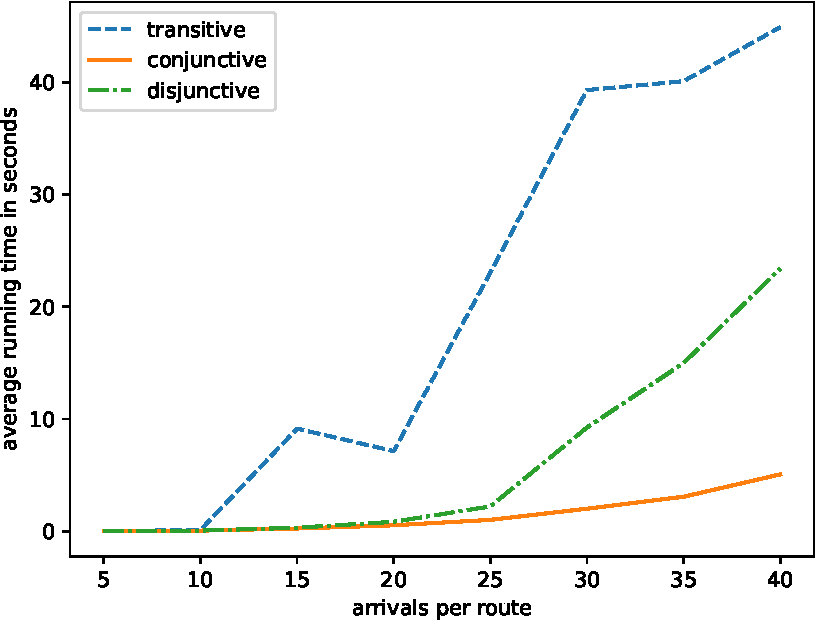
\includegraphics[width=0.7\textwidth]{data-single/running_times.pdf}
  \caption{The average (censored) running time of the branch-and-cut procedure
    is plotted as a function of the number of arriving vehicles per route, for
    each of the three indicated cutting planes. Each average is computed over
    $20$ problem instances. All instances use $\rho = 4$ and $\sigma = 1$. The arrivals
    of each of the two routes are generated using the bimodal exponential
    interarrival times with $p=0.5, \mu_{s} = 0.1, \mu_{l} = 10$. This figure
    clearly shows that the conjunctive cutting planes provide the most runtime
    improvement.}
  \label{fig:running_time}
\end{figure}

\subsection{Local search}

Without relying on systematic search methods like branch-and-bound, we can try
to use some kind of local search. Specifically, compute a solution using one of
the methods from the previous section and then explore some \textit{neighboring
  solutions}, that we define next.

As seen in the previous sections, vehicles of the same route occur mostly in
groups, to which we will refer as \textit{platoons}. For example, consider for example
the route order $\eta = (0, 1, 1, 0, 0, 1, 1, 1, 0, 0)$. This example has 5
platoons of consecutive vehicles from the same route. The second platoon
consists of two vehicles from route 1.
%In general, let $P(\eta)$ denote the total number of platoons in $\eta$.
The basic idea is to make little changes in these platoons by moving vehicles at
the start and end of a platoon to the previous and next platoon of the same
route.
%
More precisely, we define the following two types of modifications to a route
order. A \textit{right-shift} modification of platoon $i$ moves the last vehicle of this
platoon to the next platoon of this route. Similarly, a \textit{left-shift} modification
of platoon $i$ moves the first vehicle of this platoon to the previous platoon
of this route.
%
We construct the neighborhood of a solution by performing every possible
right-shift and left-shift with respect to every platoon in the route order. For
illustration purposes, we have listed a full neighborhood for some example route
order in Table~\ref{tab:local_search}.

Now using this definition of a neighborhood, we must specify how the search
procedure visits these candidates.
In each of the following variants, the value of each neighbor is always computed.
%
The most straightforward way is to select the single best candidate in the
neighborhood and then continue with this as the current solution and compute its
neighborhood. This procedure can be repeated for some fixed number of times.
Alternatively, we can select the $k$ best neighboring candidates and then
compute the combined neighborhood for all of them. Then in the next step, we
again select the $k$ best candidates in this combined neighborhood and repeat.
The latter variant is sometimes referred to as \textit{beam search}.

\newcommand*{\1}{{\color{blue}1}}%
\newcommand*{\0}{{\color{red}0}}%

\begin{table}
\caption{Neighborhood of route order $\eta = (\0, \1, \1, \0, \0, \1, \1, \1, \0, \0)$.}
\label{tab:local_search}
\begin{center}
\begin{tabular}{c|c|c}
  platoon id  & left-shift & right-shift \\
  1 &  & (\1, \1, \0, \0, \0, \1, \1, \1, \0, \0) \\
  2 & (\1, \0, \1, \0, \0, \1, \1, \1, \0, \0) & (\0, \1, \0, \0, \1, \1, \1, \1, \0, \0) \\
  3 & (\0, \0, \1, \1, \0, \1, \1, \1, \0, \0) & (\0, \1, \1, \0, \1, \1, \1, \0, \0, \0) \\
  4 & (\0, \1, \1, \1, \0, \0, \1, \1, \0, \0) & (\0, \1, \1, \0, \0, \1, \1, \0, \0, \1) \\
  5 & (\0, \1, \1, \0, \0, \0, \1, \1, \1, \0) &
\end{tabular}
\end{center}
\end{table}

\section{Learning to schedule}

% autoregressive modeling
Methods that rely on the branch-and-cut framework are guaranteed to find an
optimal solution, but as we showed in Section~\ref{sec:runtime}, the running
time scales very poorly when increasing instance sizes. For this reason, we are
interested in developing heuristics to obtain good approximations in limited
time.
%
Specifically, we will consider heuristics in terms of autoregressive
models~\cite{tomczakDeepGenerativeModeling2024}.

% choose disjunctive constraints -> linear program
\paragraph{Equivalent representations of schedules}
Observe that the space of feasible solutions
of~\eqref{eq:crossing_time_scheduling} can be reduced to finitely many decisions
regarding the disjunctive constraints~\eqref{eq:disjunctive}. Specifically, each
feasible schedule $y$ can be written as the solution to some linear program
\begin{align*}
  \min_{y} \quad & \sum_{i \in \mathcal{N}} y_{i} \\
  \text{s.t.} \quad & a_{i} \leq y_{i} & \text{ for all } i \in \mathcal{N}, \\
           & y_{i} + \rho \leq y_{j}, & \text{ for all } (i,j) \in \mathcal{C}, \\
           & y_{i} + \sigma \leq y_{j}, & \text{ for all } (i,j) \in \mathcal{O} ,
\end{align*}
for some selection $\mathcal{O}$ of the disjunctive constraints. To see when
such a selection is allowed, we can think of this linear program as a weighted
directed graph on nodes $\mathcal{N}$ with conjunctive arcs
$(i,j) \in \mathcal{C}$ with weights $w(i,j) = \rho$ and disjunctive arcs
$(i,j) \in \mathcal{O}$ with weights $w(i,j) = \sigma$. Now observe that the
definition of $y$ through the linear program is equivalent to defining $y$
through
\begin{align}
  \label{eq:y_max}
  y_{j} = \max\{ a_{j}, \max_{i \in \mathcal{N}^{-}(j)} y_i + w(i,j) \} ,
\end{align}
where $\mathcal{N}^{-}(j)$ denotes the set of in-neighbors of node $j$. It is
now easy to see that $y$ is well-defined if and only if the so-called
\textit{complete disjunctive graph}
$G=(\mathcal{N}, \mathcal{C} \cup \mathcal{O})$ is acyclic.
%
When $G$ is acyclic, there is a unique topological ordering of its nodes. Hence,
any valid selection $\mathcal{O}$ of disjunctive constraints is equivalent to a
sequence $\pi$ of vehicles. It is also equivalent to a sequence $\eta$ of
routes, because the ordering of vehicles on the same route is already fixed.
From now on, we will mainly be working with $\eta$, because it is in some sense
the simplest representation of a schedule and we write $y^{\eta}$ to denote the
induced crossing times.

\paragraph{Autoregressive modeling of schedules}
Given some problem instance $s$, we now want to model the sequence $\eta$ such
that $y^{\eta}$ is an optimal schedule. To this end, we model the conditional
probability of $\eta$ given $s$ by considering autoregressive models of the form
\begin{align}
  \label{eq:autoregressive}
  p(\eta | s) = \prod_{t=1}^{N} p(\eta_{t} | s, \eta_{1:t-1}) ,
\end{align}
where $N$ denotes the total number of vehicles. Now consider some distribution
of problem instances $\mathcal{X}$, then our goal is to minimize the expected
value
\begin{align*}
  \mathbb{E}_{s \sim \mathcal{X}, \eta \sim p(\eta | s)} L(s, \eta) ,
\end{align*}
of the total vehicle delay
\begin{align*}
  L(s, \eta) = \sum_{i \in \mathcal{N}} y^{\eta}_{i} - a_{i} .
\end{align*}
%
For inference, we would ideally want to calculate the maximum likelihood
estimator
\begin{align*}
  \arg\max_{\eta} p(\eta | s) ,
\end{align*}
but this is generally very expensive to compute, because this could require
$O(|\mathcal{R}|^{N})$ evaluations of $p(\eta_{t} | s, \eta_{1:t-1})$ when we do
not make additional structural model assumption. Therefore, one often uses
\textit{greedy rollout}, which means that we pick $\eta_{t}$ with the highest
probability at every step.
% other inference methods
Other inference strategies have been proposed in the context of modeling
combinatorial optimization problems, see for example the ``Sampling'' and
``Active Search'' strategies in the seminal
paper~\cite{belloNeuralCombinatorialOptimization2017}.

% Instead of trying to map a problem instance directly to some optimal route
% order, we construct it in a step-by-step fashion. At every step, the partial
% route order induces a partial vehicle ordering, which is a permutation of the
% set of scheduled vehicles.
%
% It may be helpful to model this process as a finite-state automaton, where the
% set of route indices acts as the action space\footnote{We will later define a
%   reward, which turns the automaton into a deterministic Markov decision
%   process, so we find it more natural to say ``action space'' instead of the
%   common terminology ``input alphabet''.} $\mathcal{R} = \{ 1, \dots, n \}$. Let $S$
% denote the state space and let $\delta: S \times \mathcal{R} \rightarrow S$ denote the transition
% function.
% % states
% Let $s$ denote an instance of crossing time scheduling
% problem~\eqref{eq:crossing_time_scheduling}. We consider $s$ to be a fixed part
% of the state, so it does not change with transitions. The other part of the
% state is the current partial ordering $\pi_{t}$. The initial state is
% $s_{0} = (s, \varnothing)$.
% % transitions
% Let $s_{t} = (s, \pi) \in S$ denote some state and let $r \in \mathcal{R}$ be the next
% action that was chosen. Let $i$ denote the next unscheduled vehicle on route $r$,
% then the system transitions to $s_{t+1} = (s, \pi \mdoubleplus i)$, where
% $\mdoubleplus$ denotes sequence concatenation. If there was no next unscheduled
% vehicle $i$, the transition is undefined.
% %
% Suppose that we have some mapping $p : S \rightarrow \mathcal{R}$ to determine the next
% route, the final state can be determined by recursively computing
% \begin{align*}
%   s_{t} = \delta(s_{t-1}, p(s_{t-1})) .
% \end{align*}
%
% The goal is now to find a mapping $p$ such that the final state
% $s_{N} = (s, \pi^{*})$ correspond to some optimal ordering $\pi^{*}$.
%
% Observe that such a mapping must exist, because we can always set
% $p(s_{t}) = \eta^{*}_{t+1}$ for every step $t$, given some optimal route order
% $\eta^{*}$. However, we do not hope to find an explicit representation of $p$,
% because it would in general be very complex, so our aim is to find good
% approximations.

% multi-step transition
% With a little abuse of notation, let $\delta(s, \eta) = \delta(s_{0}, \eta)$ denote the
% state that we obtain after applying sequence $\eta$ to the automaton with initial
% state $s_{0} = (s, \varnothing)$, which generalizes the single step transition function by
% recursively defining
% \begin{align*}
%   \delta(s_{0}, \eta_{1:t}) = \delta(\delta(s_{0}, \eta_{1:t-1}), \eta_{t}) .
% \end{align*}
%
% Therefore, an input sequence $\eta$ of routes is called a \textit{valid route
%   order} whenever it is of length
% \begin{align*}
%   N = \sum_{r \in \mathcal{R}} n_{r}
% \end{align*}
% and contains precisely $n_r = |\{ i \in \mathcal{N} : r(i) = r \}|$ occurrences
% of route $r \in \mathcal{R}$.

\subsection{Model parameterization}

We can consider different ways of parameterizing $p(\eta | s)$ in terms of
$p(\eta_{t+1} | s, \eta_{1:t})$. Here, each partial sequence $\eta_{1:t}$
represents some partial schedule, which can equivalenty be defined in terms of
the sequence of \textit{scheduled} vehicles $\pi_{1:t}$. However, it is more
convenient to define a partial schedule in terms of the \textit{partial
  disjunctive graph} $G_{t} = (\mathcal{N}, \mathcal{C} \cup \mathcal{O}_{t})$,
which is defined by the unique selection $\mathcal{O}_{t}$ such that for each
$i \in \pi_{1:t}$ and each $\{i, j\} \in \mathcal{D}$, we have either
$(i, j) \in \mathcal{O}_{t}$ or $(j, i) \in \mathcal{O}_{t}$ with
$j \in \pi_{1:t}$.
%
To emphasize this parameterization in terms of the partial disjunctive graph, we
can alternatively write~\eqref{eq:autoregressive} as
\begin{align*}
  p(\eta | s) = \prod_{t=1}^{N} p(\eta_{t} | G_{t-1}) .
\end{align*}

There is a natural extensions of expression~\eqref{eq:y_max} for partial
disjunctive graphs. Given $G_{t}$, let the \textit{earliest crossing time} of
each vehicle $i \in \mathcal{N}$ be recursively defined as
\begin{align*}
  \beta_{t}(j) = \max\{ a_{j}, \max_{i \in \mathcal{N}^{-}_{t}(j)} \beta_{t}(i) + w(i,j) \} ,
\end{align*}
where $\mathcal{N}^{-}_{t}(j)$ denotes the set of in-neighbors of node $j$ in
$G_{t}$.
%
For empty schedules, we have $\beta_{0}(i) = a_{i}$ for all $i$. For complete
schedules, we have $\beta_{N}(i) = y^{\eta}(i)$ for all $i$. We have
$\beta_{t}(i) \leq \beta_{t+1}(i)$ for all $i$, because
$\mathcal{O}_{t} \subset \mathcal{O}_{t+1}$. Hence, $\beta_{t}$ can be
interpreted as providing the best lower bounds $\beta_{t}(i) \leq y^{\eta}(i)$,
regardless of how the partial schedule is completed.

\subsubsection{Threshold heuristic}

We know from Proposition~\ref{prop:exhaustive} that whenever it is possible to schedule a vehicle
immediately after its predecessor on the same route, then this must be done in
any optimal schedule.
%
Based on this idea, we might think that the same holds true whenever a vehicle
can be scheduled \textit{sufficiently} soon after its predecessor. Although this is not
true in general, we can define a simple heuristic based on this idea.

In this case, the model does not specify a distribution over $\eta$, but selects
a single candidate by selecting a single next route in each step, so with
$\mathds{1}\{ \cdot \}$ denoting the indicator function, we have
$p(\eta_{t+1} | G_{t}) = \mathds{1}\{ \eta_{t+1} = p_{\tau}(G_{t}) \}$,
selecting the next route at step $t$ as
% For every route $r \in \mathcal{R}$, let $k(r)$ denote the number of vehicles that
% have already been scheduled. Hence, let $i = (\eta_{t}, k(\eta_{t}))$ denote the
% vehicle that was scheduled in the last step.
\begin{align*}
  p_{\tau}(G_{t}) = \begin{cases}
                \eta_{t} \quad &\text{ if } \beta_{t}(\pi_{t}) + \rho + \tau \geq a_{j} \text{ and } (\pi_{t},j) \in \mathcal{C} , \\
                \texttt{next}(\eta_{t}) & \text{ otherwise, }
              \end{cases}
\end{align*}
where $\texttt{next}(\eta_{t})$ denotes some arbitrary route other than $\eta_{t}$ with
unscheduled vehicles left.
%
This definition is illustrated in Figure~\ref{fig:threshold_heuristic}.

\begin{figure}
  \centering
  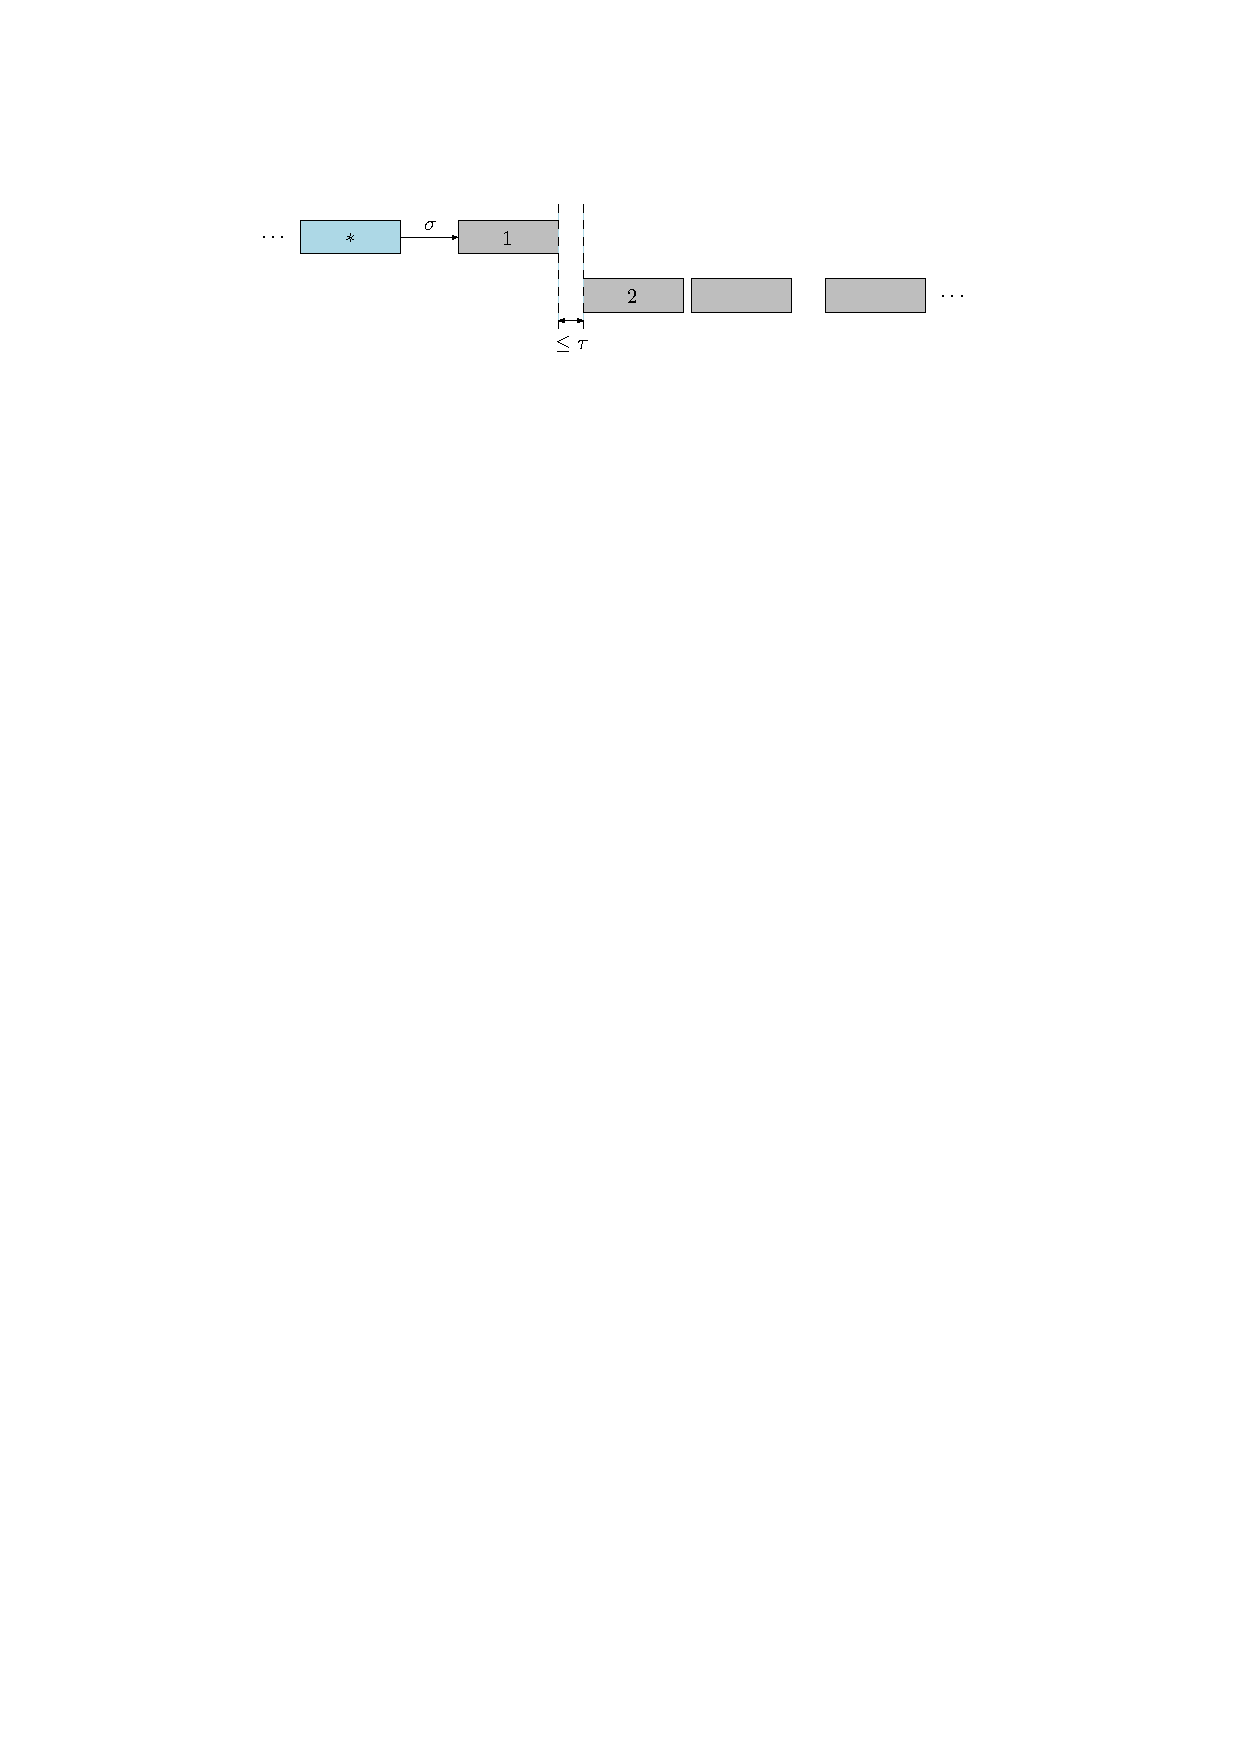
\includegraphics[width=0.8\textwidth]{figures/single/threshold}
  \caption{Illustration of how the threshold heuristic is evaluated at some
    intermediate step $t$ to choose the next route $\eta_{t+1}$. The top and
    bottom row contains the unscheduled vehicles from route 1 and route 2,
    respectively, drawn at their earliest crossing times $\beta_{t}(i)$. The
    middel row represents the current partial schedule. Vehicle $\pi_{t-1}$ is
    from route 1 and the last scheduled vehicle $\pi_{t}$ is from route 2 and
    the disjunctive constraint for them happens to be tight in this case,
    illustrated by the arrow. Whenever the indicated distance is smaller than
    $\tau$, the threshold rule selects vehicle $*$ to be scheduled next. Otherwise,
    vehicle $\dagger$ will be chosen.}\label{fig:threshold_heuristic}
\end{figure}


\subsubsection{Neural heuristic}
\label{sec:neural}

We will now consider a parameterizaton that directly generalizes the
threshold heuristic. Instead of looking at the earliest crossing time of the
next vehicle in the current lane, we now consider the earliest crossing
times of all unscheduled vehicles across lanes.
%
In the following definitions, we will drop the step index $t$ to avoid
cluttering the notation.
%
For every route $r$, let $\pi^{r}$ denote the sequence of unscheduled vehicles
and consider their crossing time lower bounds
$\beta(\pi^{r}) = (\beta(\pi^{r}_{1}), \beta(\pi^{r}_{2}), \dots)$. Let the
minimum crossing time lower bound among unscheduled vehicles be denoted by $T$,
then we call
$h_{r} = \beta(\pi^{r}) - T = (\beta(\pi^{r}_{1}) - T, \beta(\pi^{r}) - T, \dots)$
the \textit{horizon} of route $r$.

Next, we define some neural embedding $\bar{h}_{r}$ of each horizon. Observe
that horizons can be variable length. We could fix the length by using padding,
but this can be problematic for states that are almost done. Therefore, we
employ a recurrent neural network. Each horizon $h_r$ is simply transformed into
a fixed-length embedding by feeding it in reverse order through a plain Elman
RNN. Generally speaking, the most recent inputs tend to have greater influence
on the output of an RNN, which is why we feed the horizon in reverse order, such
that those vehicles that are due first are processed last, since we expect those
should have the most influence on the decision. These horizon embeddings are
arranged into a vector $h_{t}$ by the following cycling rule. At position $k$ of
vector $h_{t}$, we put the embedding for route
\begin{align*}
  k - \eta_{t} \; \mathrm{mod} \; |\mathcal{R}|
\end{align*}
where $\eta_{t}$ denotes the last selected route. Using this cycling, we make sure
that the embedding of the last selected route is always kept at the same
position of the vector.
% \begin{align*}
%   {H}_{r} = \bar{h}(r - \eta_{t} \; \mathrm{mod} \; |\mathcal{R}|) ,
% \end{align*}
%
Using some fully connected neural network $f_{\theta}$ and a softmax layer, this
global embedding is then finally mapped to a probability distribution as
\begin{align*}
  p_{\theta}(\eta_{t+1} | G_{t}) = \text{softmax} ( f_{\theta}(h_{t})) ,
\end{align*}
where $\theta$ denotes the parameters of $f$ and of the recurrent neural
networks.
% inference
After $\theta$ has been determined, we can apply greedy rollout by simply
ignoring routes that have no unscheduled vehicles left and take the argmax of
the remaining probabilities.

\begin{figure}
  \centering
  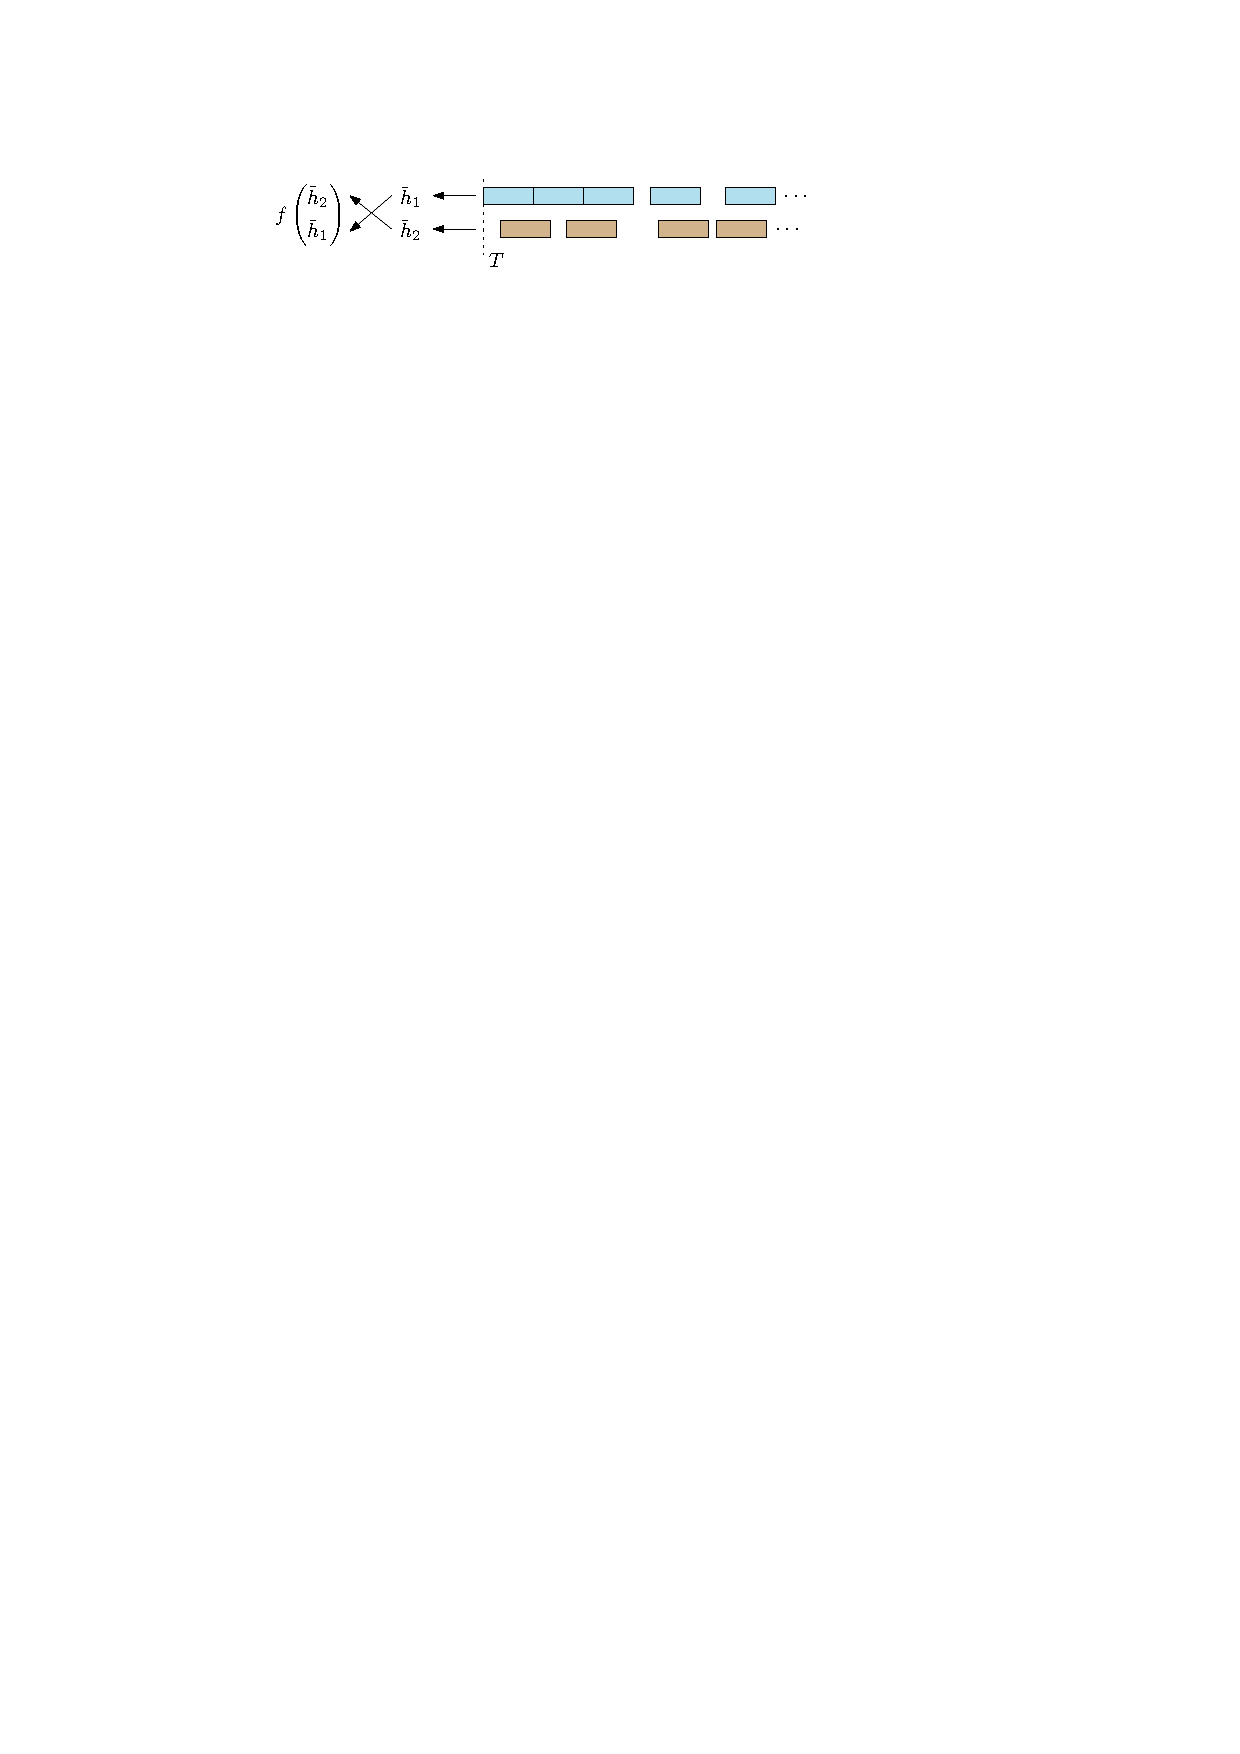
\includegraphics[width=0.8\textwidth]{figures/single/embedding}
  \caption{Schematic overview of parameterization of the neural heuristic. The
    distribution over the next route is parameterized as
    $p_{\theta}(\eta_{t+1} | G_{t})$, which is computed from the current route horizons
    $h_{r}$ via embeddings $\bar{h}_{r}$ and the cyling trick. Observe that the
    particular cycling shown in the figure corresponds to a situation in which
    the current route is $\eta_{t} = 2$.}\label{fig:neural_embedding}
\end{figure}


\subsection{Supervised learning}

We will now explain how model parameters can be tuned using some sample of
problem instances $X \sim \mathcal{X}$.
%
Given some instance $s$, let $\eta_{\tau}(s)$ be the schedule produced by the
threshold heuristic. Note that $L(s, \eta^{\tau}(s))$ is not differentiable with
respect to $\tau$, so we cannot use gradient-based optimization methods.
However, we only have a single parameter, so we can simply select the value of
$\tau$ that minimizes the average empirical loss
%
\begin{align*}
  \min_{\tau \geq 0} \sum_{s \in X} L(s, \eta_{\tau}(s)) ,
\end{align*}
%
which can be computed through a simple grid search.
%
This approach is no longer possible when $p(\eta \, | s)$ is a proper distribution,
so we need to something different for the neural parameterization.

Consider some instance $s \in X$ and let $\eta^{*}$ denote some optimal route
sequence, which can for example be computed by solving the MILP from
Section~\ref{sec:branch-and-cut}. For each such optimal schedule, we can compute
the sequence $G_{0}, \eta_{1}, G_{1}, \eta_{2}, \dots, \eta_{N}, G_{N}$. The
resulting set of pairs $\{ (G_{t}, \eta_{t+1}) : t = 1, \dots, N - 1 \}$ can be used to
learn $p_{\theta}$ in a supervised fashion by treating it as a classification task
and computing the maximum likelihood estimator $\hat{\theta}$. Interpreting $G_{t}$
as \textit{states} and $\eta_{t+1}$ as \textit{actions}, we see that this
approach is equivalent to \textit{imitation learning} in the context of finding
policies for Markov decision processes from so-called \textit{expert
  demonstration}.
%
Let $Z$ denote the set of all state-action pairs collected from all
training instances $X$. We make the procedure concrete for the case of two
routes $\mathcal{R} = \{ 1, 2 \}$, which is slightly simpler. Let $p_{\theta}(G_{t})$
denote the probability of choosing the first route, then we can use the binary
cross entropy loss, given by
\begin{align*}
  L_{\theta}(Z) = - \frac{1}{|Z|} \sum_{(G_{t}, \eta_{t+1}) \in Z} \mathds{1}\{\eta_{t+1} = 1\} \log(p_{\theta}(G_{t})) + \mathds{1}\{\eta_{t+1} = 2\} \log(1 - p_{\theta}(G_{t})) ,
\end{align*}
where $\mathds{1}\{\cdot\}$ denotes the indicator function. Now we can simply rely on
some gradient-descent optimization procedure to minimize $L_{\theta}(Z)$ with
respect to $\theta$.

\subsection{Reinforcement learning}

% imitation learning -> RL (on/off-policy)
Instead of using state-action pairs as examples to fit the model in a supervised
fashion (imitation learning), we can also choose to use the reinforcement
learning paradigm, in which the data collection process is guided by some
policy.

% reward definition
The reinforcement learning approach depends on the definition of a reward. For
each step $G_{t-1} \xrightarrow{\eta_{t}} G_{t}$, we can define a corresponding
reward, effectively yielding a deterministic Markov decision process.
Specifically, we define the reward at step $t$ to be
\begin{align*}
  R_{t} = \sum_{i \in \mathcal{N}} \beta_{t-1}(i) - \beta_{t}(i) .
\end{align*}
Let the return at step $t$ be defined as
\begin{align*}
  \hat{R}_{t} = \sum_{k=t + 1}^{N} R_{k} .
\end{align*}
Hence, when the \textit{episode} is done after $N$ steps, the total episodic
reward is given by the telescoping sum
\begin{align*}
  \hat{R}_{0} = \sum_{t=1}^{N} R_{t} = \sum_{i \in \mathcal{N}} \beta_{0}(i) - \beta_{N}(i)  = \sum_{i \in \mathcal{N}} a_{i} - y_{i} = - L(s, \eta) ,
\end{align*}
Therefore, maximizing the episodic reward corresponds to minimizing the
scheduling objective, as desired.
%

% REINFORCE
Policy-based methods work with an explicit parameterization of the policy. The
model parameters are then tuned based on experience, often using some form of
(stochastic) gradient descent to optimize the expected total return.
%
Therefore, the gradient of the expected return
plays a central role. The
following identity is generally known as the Policy Gradient Theorem:
\begin{align*}
  \nabla \mathbb{E}_{p} \hat{R}_{0} &\propto \sum_{s} \mu_{p}(s) \sum_{a} q_{p}(s, a) \nabla p(a | s, \theta) \\
  &= \mathbb{E}_{p}\left[ \sum_{a} q_{p} (S_{t}, a) \nabla p (a | S_{t}) \right] \\
  &= \mathbb{E}_{p}\left[ \sum_{a} p(a | S_{t}) q_{p} (S_{t}, a) \frac{\nabla p (a | S_{t})}{p (a | S_{t})} \right] \\
  &= \mathbb{E}_{p}\left[ q_{p} (S_{t}, A_{t}) \frac{\nabla p (A_{t} | S_{t})}{p (A_{t} | S_{t})} \right] \\
  &= \mathbb{E}_{p} \left[ \hat{R}_{t} \log \nabla p (A_{t} | S_{t}) \right] .
\end{align*}
% \begin{align*}
%   \nabla \mathbb{E}_{a \sim p_{\theta}(a | s)} R(s, a) &= \nabla \sum_{a} p_{\theta}(a | s) R(s, a) \\
%   &= \sum_{a} \nabla p_{\theta}(a | s) R(s, a) \\
%   &= \sum_{a} p_{\theta}(a | s) \frac{\nabla p_{\theta}(a | s)}{p_{\theta}(a | s)} R(s, a) \\
%   &= \mathbb{E}_{a \sim p_{\theta}(a | s)} \left[  \frac{\nabla p_{\theta}(a | s)}{p_{\theta}(a | s)} R(s, a) \right] \\
%   &= \mathbb{E}_{a \sim p_{\theta}(a | s)} [ \nabla \log p_{\theta}(a | s) R(s, a) ] .
% \end{align*}
%
The well-known REINFORCE estimator is a direct application of the Policy
Gradient Theorem. At each step $t$, we update the parameters $\theta$ using a
gradient ascent update
\begin{align*}
  \theta \leftarrow \theta + \alpha \hat{R}_{t} \nabla \log p_{\theta}(\eta_{t} | G_{t}) ,
\end{align*}
with some fixed learning rate $\alpha$.
% add baseline to reduce variance
To reduce variance of the estimator, we can incorporate a so-called
\textit{baseline}, which is an estimate of the expected return of the current
state.
%
In the context of combinatorial optimization, the value of the baseline may be
interpreted as estimating the relative difficulty of an instance?

\subsection{Results}

The evalutation of model performance is roughly based on two aspects. Of course,
the quality of the produced solutions is important. Second, we need to take into
account the time that the algorithm requires to compute the solutions. We need
to be careful here, because we have both training time as well as inference
time for autoregressive models.
%
We study the effect of the problem instance distribution $\mathcal{X}$ by
varying the number of routes and number of arrivals per route, distribution of
interarrival times, arrival intensity per route and degree of platooning.

Let $N(s)$ denotes the total number of vehicles in instance $s$. To enable a
fair comparison across instances of various sizes, we report the quality of a
solution in terms of the average delay per vehicle $L(\eta, s) / N(s)$.
%
Given some problem instance $s$, let $\eta^{*}$ denote the schedule computed
using branch-and-bound. We use a fixed time limit of 60 seconds per instance for
the branch-and-bound procedure, in order to bound the total analysis time.
Therefore, it might be that $\eta^{*}$ is not really optimal for some of the
larger instances. Given some possibly suboptimal schedule $\eta$, we define its
\textit{optimality gap} as
\begin{align*}
  L(s, \eta) / L(s, \eta^{*}) - 1 .
\end{align*}
For each heuristic, we report the average optimality gap over all test
instances.

The performance of the threshold heuristic is evaluated based on optimal
solutions obtained using MILP in Table~\ref{tab:results1}.
%
With the specific choice $\tau = 0$, the threshold rule is related to the
so-called \textit{exhaustive policy} for polling systems, which is why we
consider this case separately. We plot the average objective for the values of
$\tau$ in the grid search, see Figure~\ref{fig:tau_fit}.

The neural heuristics is trained for a fixed number of training steps. At
regular intervals, we compute the average validation loss and store the current
model parameters. At the end of the training, we pick the model parameters with
the smallest validation loss. The results are listed in Table~\ref{tab:results2}.
%
For the neural heuristic, we plot the training and validation loss, see
Figure~\ref{fig:neural_fit}. It can be seen that the model converges very steadily in all cases.

% silent package loading


\begin{knitrout}
\definecolor{shadecolor}{rgb}{0.969, 0.969, 0.969}\color{fgcolor}\begin{table}
\centering
\caption{\label{tab:results1}Performance evaluation of the branch-and-cut (MILP) approach and the threshold heuristic for different classes of instances with two routes. The first two columns specify the instance class based on the number of vehicles $n$ per route and the type of arrival distribution for each route. These arrival distributions are chosen such that the arrival intensity is the same, only the degree of platooning varies. Performance is measured in terms of $L(s, \eta) / N(s)$, averaged over 100 test instances. The optimality gap is shown in parentheses for the heuristics.
The threshold heuristic is fitted based on 100 training instances and the optimal threshold and training time is indicated. For branch-and-cut the average inference time is indicated. Note that we used a time limit of 60 seconds for all the branch-and-cut computations.}
\centering
\resizebox{\ifdim\width>\linewidth\linewidth\else\width\fi}{!}{
\begin{tabular}[t]{cc|rr|r|rrcc|rr|r|rrcc|rr|r|rrcc|rr|r|rrcc|rr|r|rrcc|rr|r|rrcc|rr|r|rrcc|rr|r|rr}
\toprule
n & type & MILP & time & exhaustive (gap) & threshold (gap) & $\tau_\text{opt}$ & time\\
\midrule
10 & low & 5.29 & 0.05 & 9.49 (79.45\%) & 7.78 (47.08\%) & 0.95 & 3.79\\
30 & low & 8.60 & 2.01 & 12.72 (47.88\%) & 11.31 (31.49\%) & 2.65 & 21.04\\
50 & low & 11.03 & 13.78 & 16.56 (50.20\%) & 14.60 (32.41\%) & 1.95 & 51.09\\
10 & med & 4.46 & 0.06 & 7.20 (61.32\%) & 6.39 (43.15\%) & 2.50 & 3.79\\
30 & med & 6.99 & 1.88 & 9.43 (34.97\%) & 8.96 (28.29\%) & 1.10 & 21.14\\
50 & med & 8.55 & 15.11 & 11.50 (34.40\%) & 10.77 (25.93\%) & 1.70 & 51.23\\
10 & high & 4.47 & 0.06 & 6.35 (42.04\%) & 5.70 (27.51\%) & 1.35 & 3.81\\
30 & high & 6.90 & 1.90 & 8.92 (29.19\%) & 8.58 (24.25\%) & 1.00 & 21.16\\
50 & high & 7.37 & 14.99 & 9.36 (26.94\%) & 8.88 (20.42\%) & 0.80 & 51.45\\
\bottomrule
\end{tabular}}
\end{table}

\end{knitrout}



% \subsection{Regeneration theorem}

% It has been observed that some optimal schedules seem to \textit{decompose} into
% parts, whenever the crossing times of consecutive vehicles are sufficiently far
% apart~\cite{limpensOnlinePlatoonForming2023}.

% \begin{proposition}
%   Let $s$ be an instance of crossing time scheduling problem~\eqref{eq:crossing_time_scheduling}.
% \end{proposition}


\bibliography{references}
\bibliographystyle{ieeetr}


\newpage

\appendix

\section{Proof of Proposition~\ref{prop:exhaustive}}\label{app:proof}

First, we prove the following lemma that provides an easier expression for
calculating the lower bounds.

\begin{lemma}\label{lb_lemma}
  Let $\pi$ be some permutation of $\mathcal{N}$. Assume that
  $\sigma_{i} = \rho_{i} + s$, for every $i \in \mathcal{N}$, with $s > 0$.
  Consider a pair $i,j \in \mathcal{N}$ such that $i$ is the immediate predecessor
  of $j$ in $\pi$, so $\pi^{-1}(i) + 1 = \pi^{-1}(j)$, then
\begin{align}
  \label{eq:lb_lemma}
  \beta_\pi(j) = \max \{ r_{j}, \beta_\pi(i) + w(i, j) \} .
\end{align}
\end{lemma}
\begin{proof}
  Suppose $(i,j) \in \mathcal{C}$, see Figure~\ref{fig:lb_lemma},
  then the incoming disjunctive arcs of $j$ are
  $N^{-}_{\pi}(j) \setminus \{ i \} \subset N^{-}_{\pi}(i)$. Therefore, we have
  \begin{align*}
    \max_{v \in N^{-}_{\pi}(j) \setminus \{i\}} \beta_\pi(v) + \sigma_{v} \leq \beta_\pi(i) ,
  \end{align*}
  so that
      $\beta_\pi(v) + w(v,j) \leq \beta_\pi(i) + w(i,j)$
  for all $v \in N_{\pi}^{-}(j)$.

  Otherwise, we have $(i, j) \in \mathcal{O}(\pi)$.
  %
  Let $v \in \mathcal{N}$ such that $(v, j)$ is an arc.
  If $(v,j) \in \mathcal{C}$, then we have
  \begin{align*}
    \beta_\pi(v) + w(v,j) =
    \beta_\pi(v) + \rho_{v} \leq \beta_\pi(v) + \sigma_{v} + \sigma_{i} \leq \beta_\pi(i) + w(i,j) ,
  \end{align*}
  where the second inequality follows from $(v,i) \in \mathcal{O}(\pi)$.
  %
  If $(v, j) \in \mathcal{O}(\pi)$ with $r(v) \neq r(i)$, then $(v,i) \in \mathcal{O}(\pi)$, so
  \begin{align*}
    \beta_\pi(v) + w(v, j) = \beta_\pi(v) + w(v, i) \leq \beta_\pi(i) \leq \beta_\pi(i) + w(i,j) .
  \end{align*}
  If $(v, j) \in \mathcal{O}(\pi)$ with $r(v) = r(i)$, then there is a path of conjunctive arcs between $v$ and
  $i$, so we must have $\beta_\pi(v) + \rho_{v} \leq \beta_\pi(i)$.
  Furthermore, from $w(v,j) = \sigma_{v} = \rho_{v} + s$ follows that
  \begin{align*}
    \beta_\pi(v) + w(v,j) = \beta_\pi(v) + \rho_{v} + s \leq \beta_\pi(i) + s \leq \beta_\pi(i) + w(i, j) .
  \end{align*}

  To conclude, we have shown that
  $\beta_\pi(v) + w(v,j) \leq \beta_\pi(i) + w(i,j)$ for any
  $v \in N^{-}_{\pi}(j)$, from which statement~\eqref{eq:lb_lemma} follows.
\end{proof}

\begin{figure}
  \centering
  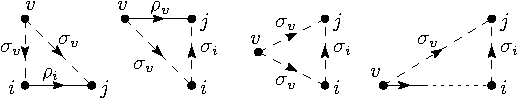
\includegraphics[width=0.9\textwidth]{figures/single/lower-bound-lemma.pdf}
  \caption{Sketch of the four cases distinguished in the proof of
    Lemma~\ref{lb_lemma}. Arc weights are given and disjunctive arcs
    $\mathcal{O}(\pi)$ are drawn with a dashed line.}\label{fig:lb_lemma}
\end{figure}


% \begin{proposition}
%   Consider an instance of~\eqref{eq:crossing_time_scheduling} with
%   $\rho_{i} = \rho$ and $\sigma_{i} = \sigma > \rho$ for all
%   $i \in \mathcal{N}$. Suppose $y$ is an optimal schedule with
%   $y_{i^{*}} + \rho \geq r_{j^{*}}$, for some $(i^{*},j^{*}) \in \mathcal{C}$,
%   then $j^{*}$ follows immediately after $i^{*}$, so
%   $y_{i^{*}} + \rho = y_{j^{*}}$.
% \end{proposition}

\Exhaustive*
\begin{proof}
  Suppose the ordering $\pi$ of $y$ is such that
  $\pi^{-1}(i^{*}) + 1 < \pi^{-1}(j^{*})$.
  %
  Let $\mathcal{I}(i,j) = \{ i, \pi(\pi^{-1}(i) + 1), \dots, j \}$ be the set of
  vehicles between $i$ and $j$.
  %
  Let $f = \pi(1)$ and $e = \pi(|\mathcal{N}|)$ be the first and last vehicles,
  respectively, and set $u = \pi^{-1}(i^{*}) + 1$ and $v = \pi^{-1}(j^{*}) - 1$, see also Figure~\ref{fig:platoon-preservation-diagram}.
  Construct new ordering $\pi'$ by moving vehicle $j^{*}$ forward
  by $|\mathcal{I}(u,v)|$ places and let $y'$ denote the corresponding schedule.
  %
  We have $y_{i} = y'_{i}$ for all $i \in \mathcal{I}(f, i^{*})$, so these do not
  contribute to any difference in the objective.
  %
  Using Proposition~\ref{prop:active-schedule} and Lemma~\ref{lb_lemma}, we compute
  \begin{align*}
    y'_{j^{*}} &= \max \{ r_{j^{*}}, y_{i^{*}} + \rho \} = y_{i^{*}} + \rho , \\
    y_{u} &= \max \{ r_{u}, y_{i^{*}} + \sigma \} , \\
    y'_{u} &= \max \{ r_{u}, y_{i^{*}} + \rho + \sigma \} ,
  \end{align*}
  where we used that $y_{i^{*}} + \rho \geq r_{j^{*}}$ by assumption.
  %
  Note that we have
  $y_{i^{*}} + \sigma + (|\mathcal{I}(u,v)| - 1) \rho \leq y_{v}$, regardless of the
  type of arcs between consecutive vehicles in $\mathcal{I}(u,v)$. Therefore,
  \begin{align*}
    y_{j^{*}} - y'_{j^{*}} \geq y_{v} + \sigma - y_{i^{*}} - \rho \geq 2 \sigma + (|\mathcal{I}(u,v)| - 2) \rho .
  \end{align*}

  We now show that $y'_{k} \geq y_{k}$ and $y'_{k} - y'_{j^{*}} \leq y_{k} - y_{i^{*}}$ for every $k \in \mathcal{I}(u,v)$.
  For $k = u$, it is clear that $y'_{u} \geq y_{u}$ and
  \begin{align*}
    y'_{u} - y'_{j^{*}} = \max \{ r_{u} - (y_{i^{*}} + \rho), \sigma \} \leq \max \{ r_{u} - y_{i^{*}}, \sigma \} = y_{u} - y_{i^{*}}.
  \end{align*}
  Now proceed by induction and let $x$ be the immediate predecessor of $k$ for
  which the inequalities hold, then
  \begin{align*}
    y'_{k} = \max \{ r_{k}, y'_{x} + w(x,k) \} \geq \max \{ r_{k}, y_{x} + w(x,k) \} = y_{k}
  \end{align*}
  and the second inequality follows from
  %\begin{align*}
  %  y'_{k} - y'_{x} = \max \{ r_{k} - y'_{x}, w(x,k) \} &\leq \max \{ r_{k} - y_{x}, w(x,k)\} = y_{k} - y_{x}
  %\end{align*}
  %implies that
  %\begin{align*}
  %  y'_{k} - y'_{j^{*}} = (y'_{k} - y'_{x}) + (y'_{x} - y'_{j^{*}}) \leq (y_{k} - y_{x}) + (y_{x} - y_{i^{*}}) = y_{k} - y_{i^{*}} .
  %\end{align*}
  %
  \begin{align*}
    (y'_{k} - y'_{x}) + (y'_{x} - y'_{j^{*}}) &= \max \{ r_{k} - y'_{x}, w(x,k) \} + (y'_{x} - y'_{j^{*}}) \\
                                             &\leq \max \{ r_{k} - y_{x}, w(x,k) \} + (y_{x} - y_{i^{*}}) \\
                                             &= (y_{k} - y_{x}) + (y_{x} - y_{i^{*}}) .
  \end{align*}

  Let $l$ denote the immediate successor of $j^{*}$, if there is one. Regardless of
  whether $j^{*}$ and $l$ are in the same lane, we have
  $y_{j^{*}} + \rho \leq y_{l}$. We derive
  \begin{align*}
    y'_{v} = y'_{v} - y'_{j^{*}} + y'_{j^{*}} \leq y_{v} - y_{i^{*}} + y'_{j^{*}} = y_{v} + \rho \leq y_{j^{*}} - \sigma + \rho ,
  \end{align*}
  from which follows that $y'_{v} + \sigma \leq y_{l}$,
  %\begin{align*}
  %  y'_{v} + \sigma = (y'_{v} - y'_{j^{*}}) + y'_{j^{*}} + \sigma \leq y_{v} - y_{i^{*}} + y'_{j^{*}} + \sigma = y_{v} + \rho + \sigma \leq y_{j^{*}} + \rho \leq y_{l} ,
  %\end{align*}
  which means that $y_{i} \geq y'_{i}$ for $i \in \mathcal{I}(l, e)$.

  We can now compare the objectives by putting everything together
  \begin{align*}
    \sum_{i \in \mathcal{N}} y_{i} - y'_{i} &=  y_{j^{*}} - y'_{j^{*}} + \sum_{i \in \mathcal{I}(u, v)} y_{i} - y'_{i} + \sum_{i \in \mathcal{I}(l, e)} y_{i} - y'_{i} \\
    &\geq 2 \sigma + (|\mathcal{I}(u,v)| - 2) \rho + \sum_{k \in \mathcal{I}(u,v)} (y_{k} - y_{i^{*}}) - (y'_{k} - y'_{j^{*}}) \\ & \hspace{12em} - |\mathcal{I}(u,v)| (y'_{j^{*}} - y_{i^{*}}) \\
    &\geq 2 \sigma - 2 \rho > 0
  \end{align*}
  which contradicts the assumption that $y$ and $\pi$ were optimal.
  %
  Finally, from Proposition~\ref{prop:active-schedule} and Lemma~\ref{lb_lemma}
  follows that $y_{i^{*}} + \rho = y_{j^{*}}$.
\end{proof}

\begin{figure}
  \centering
  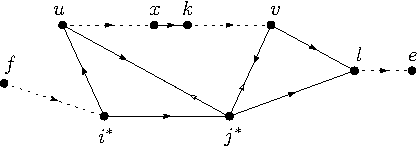
\includegraphics[width=0.8\textwidth]{figures/single/platoon-preservation-proof-diagram.pdf}
  \caption{Sketch of the nodes and most important arcs used in the proof of
    Proposition~\ref{prop:exhaustive}. Dashed arcs represent chains of
    unspecified length. The two open arrows indicate the new direction of their
    arc under ordering $\pi'$.}\label{fig:platoon-preservation-diagram}
\end{figure}


\section{Implementation details}

We have an \texttt{ActionTransform} base class with implementations
\texttt{PaddedEmbeddingModel} and \texttt{RecurrentEmbeddingModel}. The
\texttt{ActionTransform} class takes care of transforming actions in terms of
staying on the same lane or moving to the next lane to actions in terms of
absolute lane identifiers. Specifically, \texttt{action\_transform()} takes a
logit of the binary choice model and outputs a lane identifier and
\texttt{inverse\_action\_transform()} takes a lane identifier and outputs either
zero or one.
%
Both embedding models have a \texttt{state\_transform()} method that constructs a
numerical observation tensor based on the state encoded in the automaton, as
explained in Section~\ref{sec:neural}. Note that all three of the above functions are fixed,
in the sense that they do not rely on any learnable parameters. The reason for
treating these fixed parts of the model separately is that prevents us from
recomputing these transformations, because it allows us to store the transformed
state-action pairs to disk to use across different training runs.
%
Figure~\ref{fig:state-action-transforms} shows an overview of the state and action transform functions and how
they are related to each other.
%
We explicitly store the length of the
horizon as the first entry of the tensor. Maybe we should use the
\texttt{torch.nn.utils.rnn.pack\_sequence()} function that is available in
\texttt{torch}.

\begin{figure}[h]
  \centering
  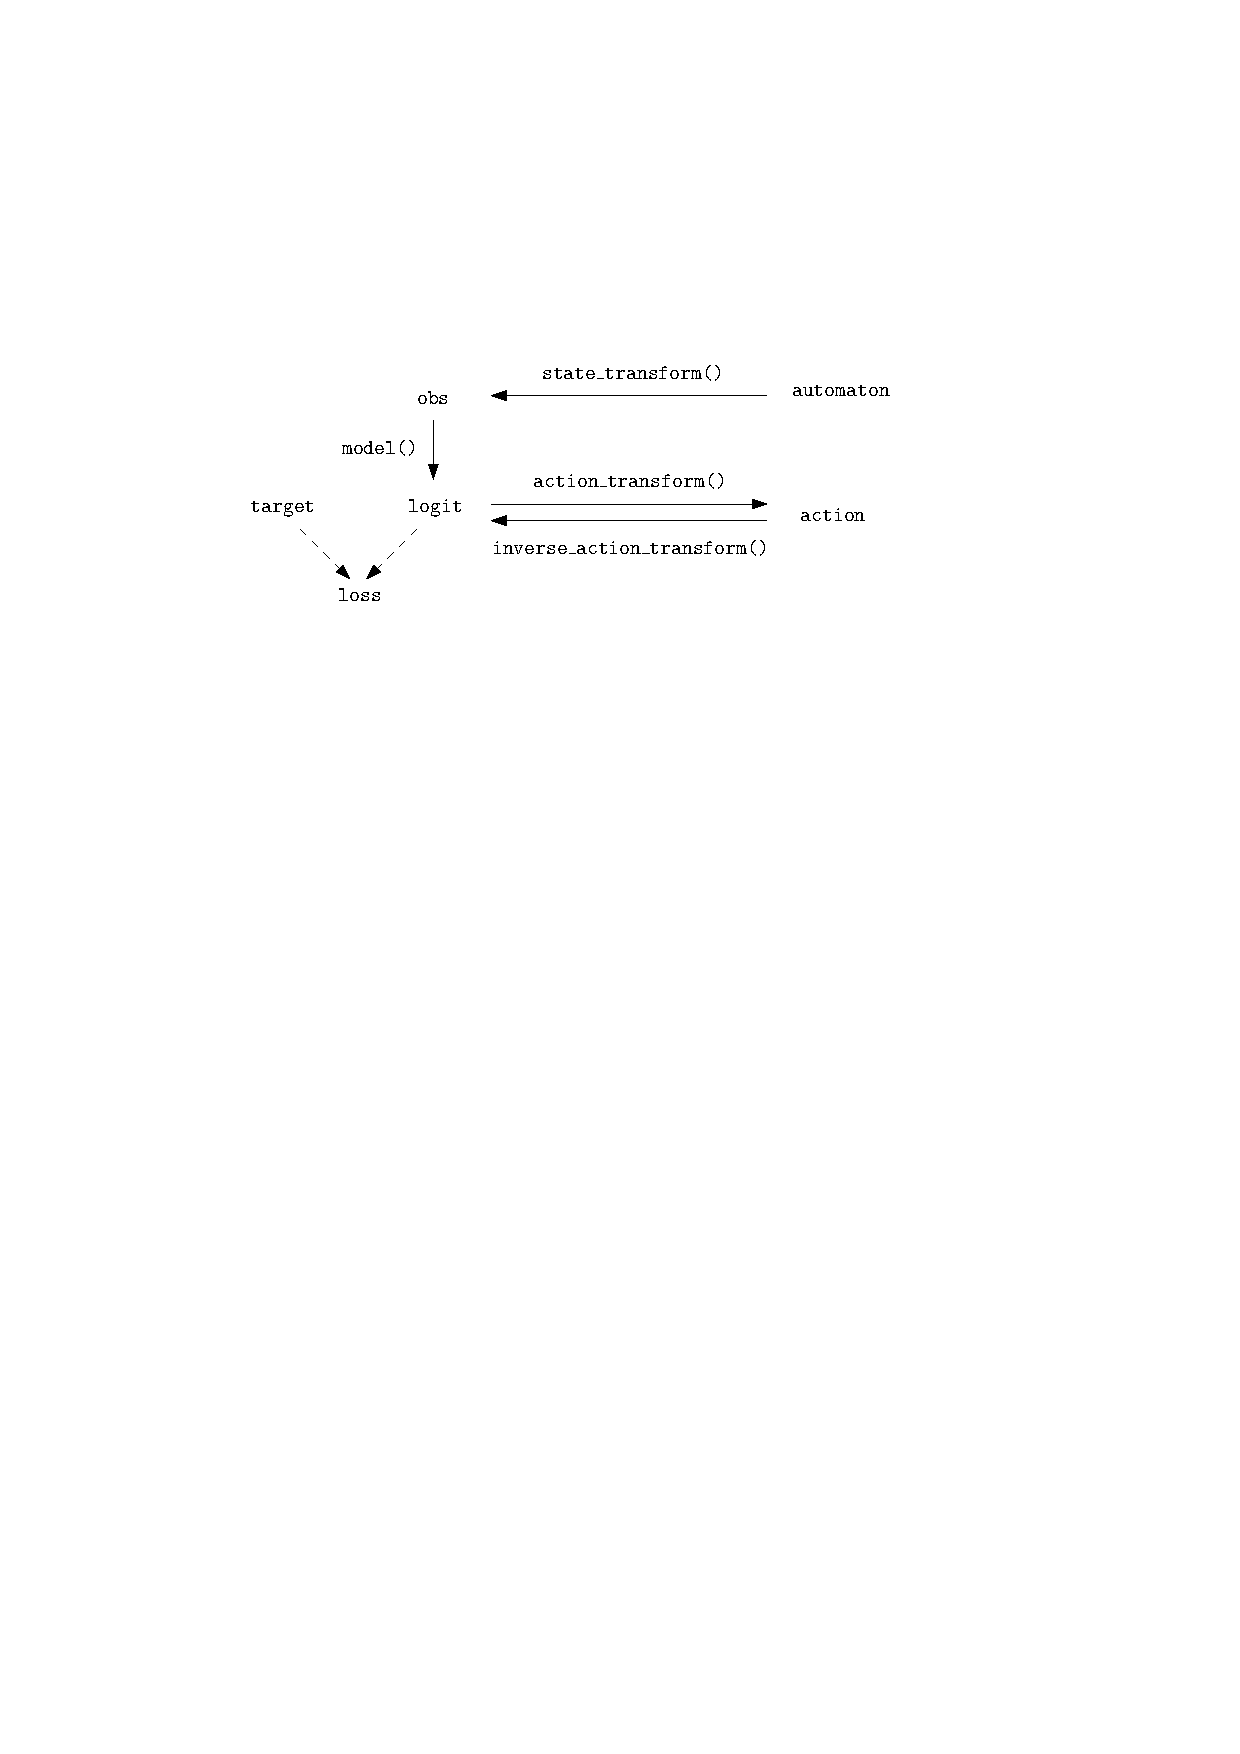
\includegraphics[scale=1]{figures/state_action_transforms}
  \caption{Schematic of the state and action transform functions used for
    imitation learning. Given some optimal state-action training pair, the
    \texttt{target} logit is computed from the optimal action using the inverse
    action transform.}
  \label{fig:state-action-transforms}
\end{figure}


\newpage


\begin{figure}
  \centering
  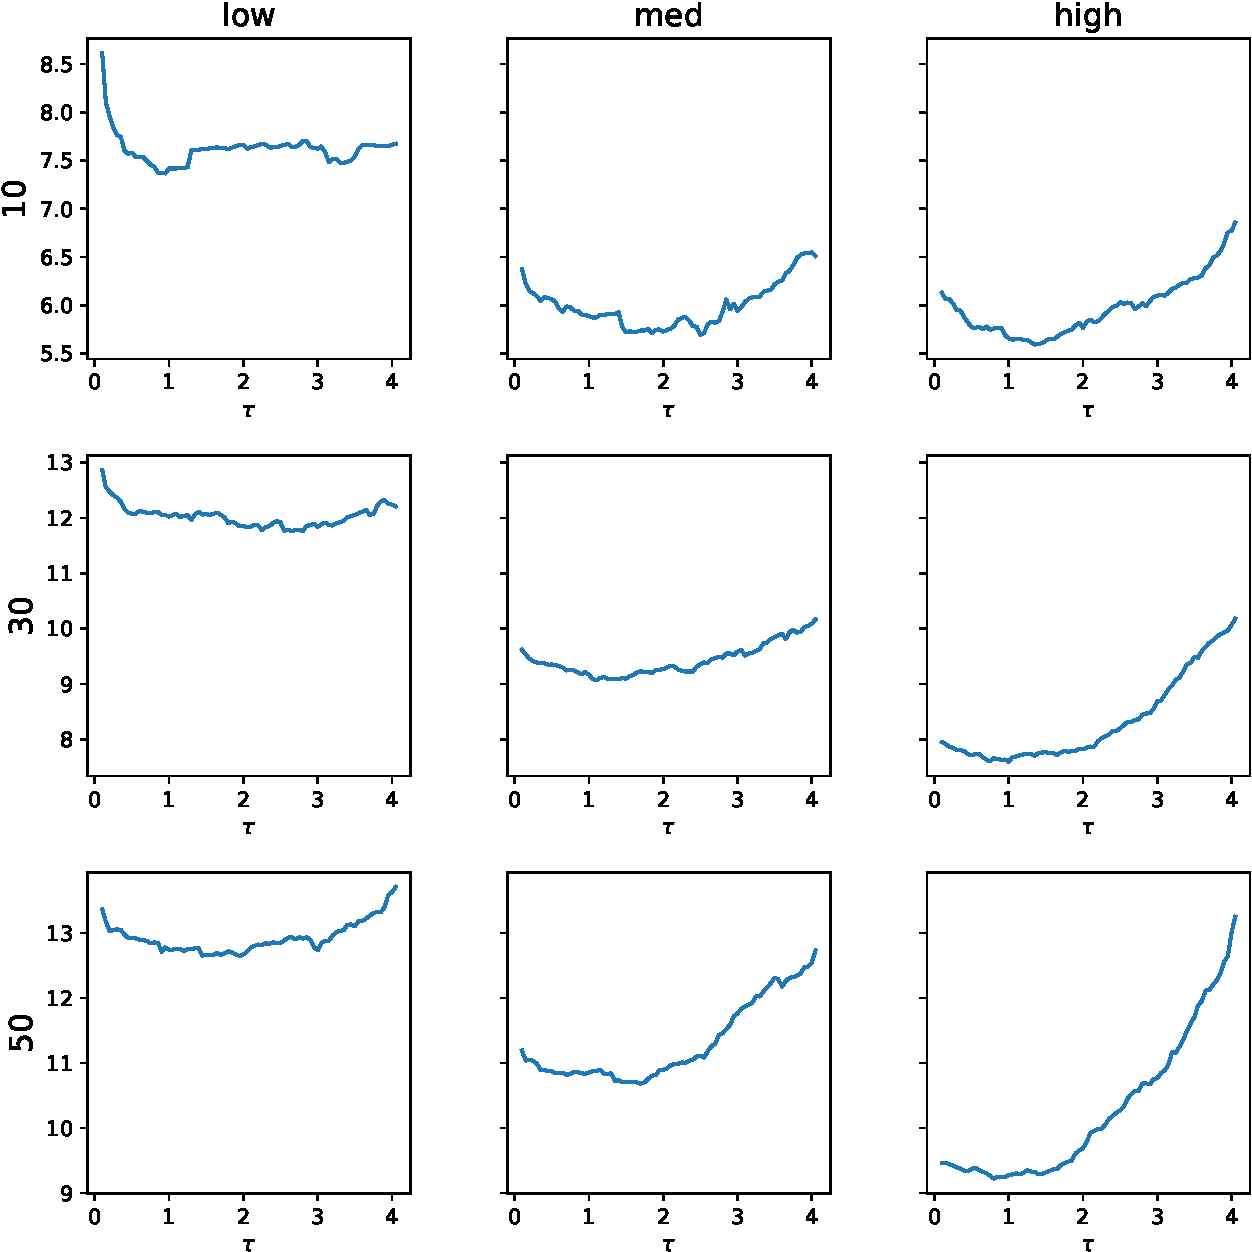
\includegraphics[width=0.9\textwidth]{figures/single/tau_fit.pdf}
  \caption{Charts to verify threshold heuristic model fit. For each indicated
    instance training set, the average delay
    $\sum_{s \in \mathcal{X}} \textrm{obj}(y_{\tau}(s)) \, / \, {|\mathcal{X}|}$
    is plotted as a function of the threshold $\tau$. We use these plots to
    verify that the range of possible candidates for $\tau$ has been chosen wide
    enough, which is probably the case when the graphs are somewhat smooth and
    convex. Observe that larger instances show smoother curves. Furthermore,
    observe that the class of instances with high arrival intensity shows an
    apparent optimal value of $\tau$ around $1$, which might be related somehow
    to our choice of $\sigma = 1$.}
  \label{fig:tau_fit}
\end{figure}

\begin{figure}
  \centering
  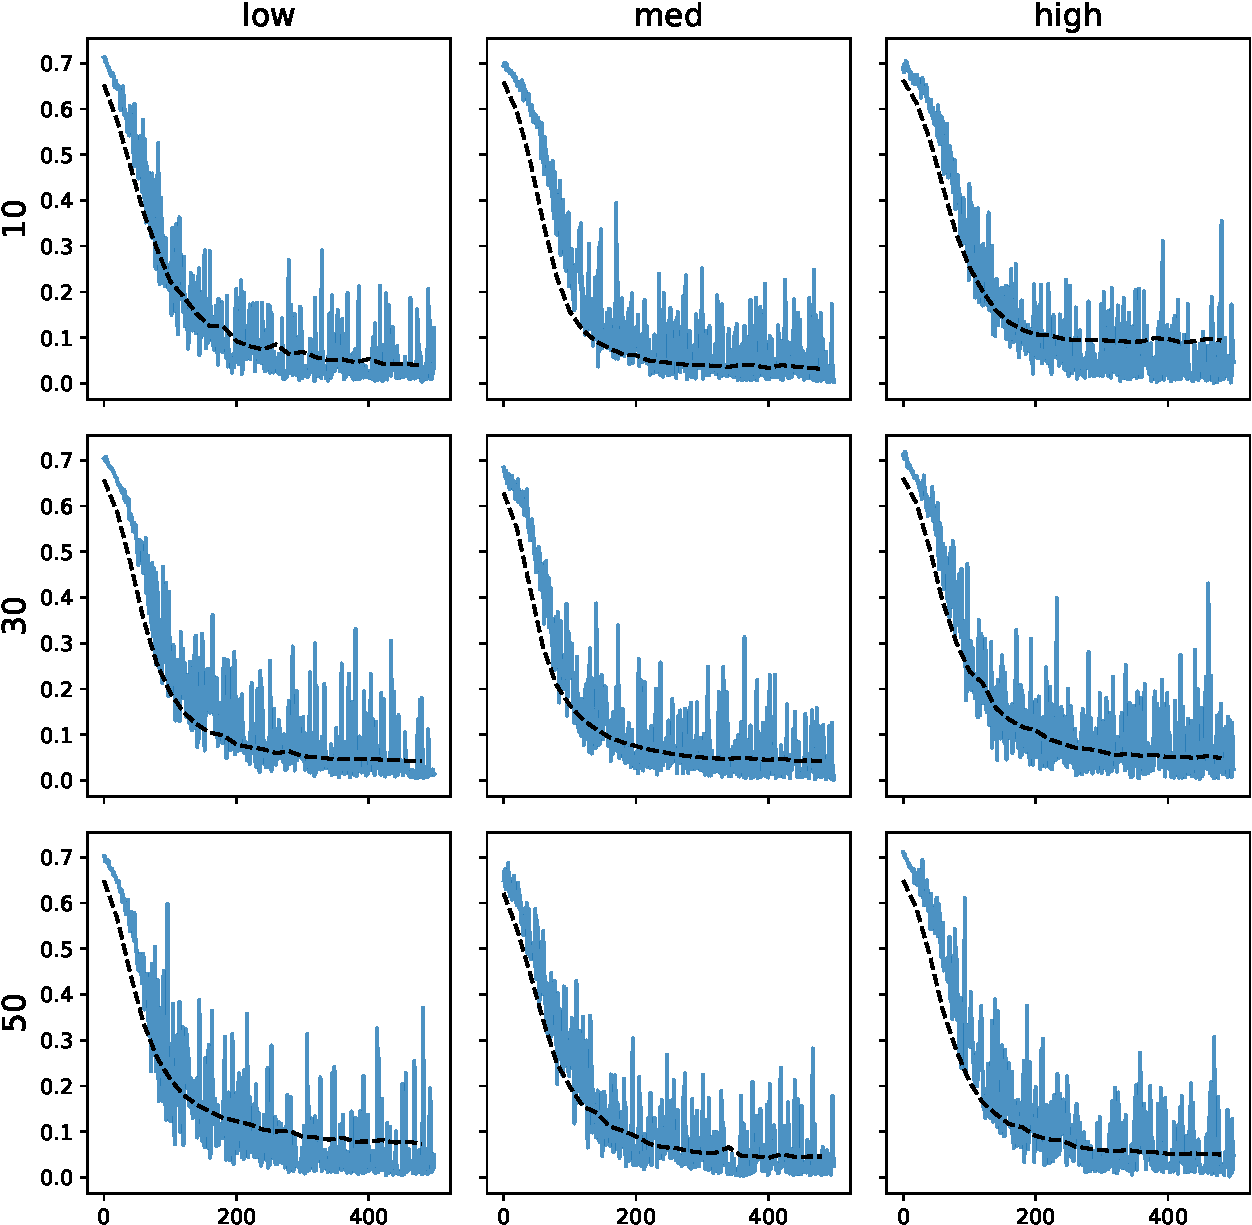
\includegraphics[width=0.9\textwidth]{figures/single/neural_fit.pdf}
  \caption{Loss plots to verify neural heuristic model fit. For each indicated
    instance training set, the training loss is plotted for each training step
    in blue and the validation loss is plotted as the dashed line. Recall that
    the validation loss is the average binary cross entropy loss after a given
    number of training steps. The training loss is plotted for each individual
    step without smooting.}
  \label{fig:neural_fit}
\end{figure}

\end{document}

% to enable the minted package
% Local Variables:
% TeX-command-extra-options: "-shell-escape"
% End:
